\documentclass[11pt]{article}
% Language setting
% Replace `english' with e.g. `spanish' to change the document language
\usepackage[spanish]{babel}

% Set page size and margins
% Replace `letterpaper' with`a4paper' for UK/EU standard size
\usepackage[a4paper,top=1.9cm,bottom=2.2cm,left=1.9cm,right=1.32cm,marginparwidth=1.75cm]{geometry}

\setlength{\parindent}{1em}
\setlength{\parskip}{1em}

% Useful packages
\usepackage{amsmath}
\usepackage{mathtools}
\usepackage{graphicx}
\usepackage{xcolor}
% \usepackage{color}% xcolor or color
\usepackage[colorlinks=true, allcolors=blue]{hyperref}

% Set document Font
\usepackage{fontspec}

\setmainfont{Times New Roman}

% Para las ecuaciones: https://latex.codecogs.com/eqneditor/editor.php?lang=es-es

\title{
	Proyecto Global Integrador:
	\\
	Control Semi-Automático Coordinado de Grúa Portuaria de Muelle tipo Pórtico
}

\author{
	Guarise Renzo
	\\
	Trubiano Lucas
	\\
	Profesor: Ing. Gabriel L. Julián
	\\
	\\
	Autómatas y Control Discreto
	\\
	Ingeniería Mecatrónica
	\\
	Universidad Nacional de Cuyo - Facultad de Ingeniería
}

\begin{document}
\maketitle

\begin{center} % Centrar texto
    {\Large \textbf{Resumen}}
\end{center}

Este informe presenta el proyecto de un control semi-automático coordinado de una grúa portuaria de muelle tipo pórtico, desarrollado con Matlab, Simulink, Stateflow y CODESYS. El objetivo del proyecto es diseñar un sistema de control multinivel (Nivel 0, 1 y 2) que permita la coordinación entre las distintas funciones de la grúa, mejorando la eficiencia y seguridad en la carga y descarga de contenedores en el puerto.
\par
Para esto consideraremos unas simplificaciones en el sistema físico; en primer lugar vamos a suponer un movimiento en 2 dimensiones en los ejes ``x'' e ``y'', tanto del contenedor como del carro; consideramos que luego este movimiento se replicaría en cada carril; en segundo lugar para moverse en el plano tendremos en cuenta 2 tipos de movimiento uno de avance/retroceso del carro y otro de izaje del cable y la carga, lo que supone un movimiento de tipo péndulo del contenedor. Dichas simplificaciones sirven para el planteo del modelo matemático y físico de la planta. Luego se verán más adelante otras simplificaciones realizadas como consideraciones de estructuras rígidas, etc.
\par
Las fases de desarrollo del proyecto se dividen en 2, “Model-in-the-loop” y “Software-in-the-loop”. La primera consta de usar Matlab, Simulink y Stateflow para construir un modelo del sistema y el sistema de control, y realizar pruebas y simulaciones para determinar el correcto funcionamiento de los mismos. Luego la segunda etapa consta de llevar la lógica del autómata a un entorno estandarizado como CODESYS (según norma IEC 61131-3) y realizar una prueba conjunta con comunicación por protocolo OPC UA para verificar el correcto funcionamiento del automatismo y la planta.



% \tableofcontents % Creamos el indice
\newpage
\section{Introducción}


Una de las formas más comunes de comercializar y mover productos y/o materias primas en grandes cantidades es a través de contenedores en barcos. Esto se ha difundido de tal forma en el mundo que los puertos son claves para las economías de los países. En estos puertos se mueven grandes cantidades de contenedores, en tiempos muy reducidos por lo cuál la eficiencia y la productividad son aspectos esenciales del control, y teniendo en cuenta que son objetos de gran tamaño y peso, tenemos que tener en cuenta los riesgos que esto implica y debemos crear sistemas de control que puedan manipularlos con una alta precisión y seguridad. Para esto se utilizan grúas que son semi-automáticas, es decir, tramos con operación manual y tramos con operación automática. A estas grúas se les dota de sistemas de control lo suficientemente robustos y a prueba de fallas.
\par
Para resolver este problema lo primero es realizar el modelado físico que, por simplificación, consta de un carro en la parte superior que es tirado por un sistema de cables cerrados a ambos lados del mismo y hacen que se mueva en dirección horizontal. Del mismo cuelga un cable que sostiene el spreader+contenedor, este cable se puede izar, de tal forma que, también simplificando el modelo, el sistema queda como el de un carrito con un péndulo de longitud variable. Del extremo del cable cuelga un ``spreader'' que sostiene el contenedor y esto conforma la carga del péndulo o del cable.
\par
Luego de resolver el modelado físico-matemático del sistema procedemos a desarrollar un autómata que tiene funciones de control y seguridad y está formado por 3 niveles:
\begin{itemize}
    \item \textbf{Nivel 2:} Este controlador está compuesto por otros dos controladores de estados continuos en tiempo discretizado (controles de lazo cerrado PID), estos reciben consignas del controlador superior (Nivel 1) separado por 2 consignas, una de izaje y otra de traslación del carro. En base a dichas consignas planteamos un control genérico de 4 cuadrantes sobre los accionamientos electromecánicos. Los controladores son unos PID de movimiento con modulador de torque para izaje y traslación, y control tipo PD para el balanceo.
    \item \textbf{Nivel 1:} Es un controlador de estados discretos activado por eventos. Su estructura es jerárquica y concurrente para una mejor performance de las trayectorias. 
    \item \textbf{Nivel 0:} Este nivel es un control también de estados discretos activado por eventos, que se encarga de detectar condiciones de operación inseguras para proteger al sistema y asegurar la confiabilidad del mismo o actuar en casos de fallas y/o colisiones.
\end{itemize}
\par
Estos controladores de los 3 niveles fueron desarrollados primero en Stateflow y Simulink (componentes de Matlab) para facilitar el desarrollo, testeo y simulación de su funcionamiento; ya que estas herramientas del ecosistema de Matlab son fáciles de integrar. Así cuando se verificó que estaba bien el desarrollo y que el funcionamiento cumplía con los requerimientos se implementó esa misma lógica en el entorno de desarrollo industrial CODESYS, siguiendo la norma IEC 61131-3.


\newpage


\section{Desarrollo}
Como se mencionó anteriormente, el desarrollo de este proyecto requiere un enfoque sistemático y riguroso. Para seguir este enfoque, lo primero que se debe hacer es obtener un \textbf{modelo físico-matemático} preciso y detallado que permita modelar y simular el sistema de la grúa de la forma más exacta posible, teniendo en cuenta las simplificaciones e hipótesis necesarias para hacer el modelo que mejor represente nuestro sistema.
\par
Una vez que se tiene dicho modelo, avanzamos al siguiente paso que es: diseñar y optimizar el \textbf{sistema de control}. Este sistema de control es el corazón del proyecto, y se encarga de garantizar que la grúa se mueva con precisión, eficiencia y seguridad en todo momento. Para hacer esto, se deben llevar a cabo simulaciones exhaustivas para identificar y resolver cualquier problema potencial antes de pasar al siguiente paso.
\par
Con el sistema de control diseñado y optimizado, pasamos a la fase de prueba. Aquí, el autómata se convierte en código usando la plataforma de programación \textbf{CODESYS} y se simula el funcionamiento completo del sistema. Se evalúan el rendimiento y la precisión del sistema en condiciones de operación, y se realiza una evaluación rigurosa para garantizar que el sistema cumpla con todas las especificaciones requeridas.
\par
Finalmente, se presentan los \textbf{resultados} obtenidos y las \textbf{conclusiones} finales. Aquí se discuten los logros del proyecto, se identifican las lecciones aprendidas y se destacan los aspectos a mejorar.

\section{Modelado del sistema}

El sistema se compone de dos movimientos fundamentales, el \textbf{sistema de traslación horizontal (carro)}, y el \textbf{sistema movimiento vertical (izaje)}. Vamos a desarrollar las ecuaciones de ambos sistemas por separado y luego veremos cómo esos movimientos se combinan para dar como resultado las ecuaciones de movimiento del contenedor en el \textbf{plano x-y}.

\subsection{Hipotesis}
El sistema real planteado es de una complejidad considerable, por lo cuál, para los fines académicos vamos a plantear una serie de simplificaciones o consideraciones sobre el modelo:
\begin{itemize}
	\item Consideraremos a la estructura del pórtico completamente rígida.
	\item El carro que se desliza sobre la estructura, tiene un desplazamiento puramente horizontal y sin resbalamiento. Es tirado por cables a ambos lados del carro en un sistema cerrado que es movido por unos tambores ubicados en la casa de máquinas.
	\item Los mecanismos de transmisión del carro se consideran rígidos.
	\item Consideramos un único cable de acero equivalente de carro siempre tensado (a tracción), con elasticidad longitudinal amortiguada.
	\item Asumimos mecanismo equivalente (1 tambor con 1 freno de emergencia, 1 motor con 1 freno).
	\item El cable de acero equivalente de izaje, tiene masa propia despreciable, elástico sólo a tracción (no soporta compresión).
	\item Vamos a suponer que no existen efectos externos sobre el carro ni la carga. Es decir, no hay efectos aerodinámicos al chocar con el viento.
	\item El sistema está sometido a la acción de la aceleración de la gravedad, que se aplica verticalmente sobre la carga. Y también a la interacción de contacto o apoyo de la carga o spreader sobre el suelo.
\end{itemize}

\subsection{Sistema de traslación del carro}
\label{section:carro}

Teniendo en cuenta el primer sistema de movimiento. El carro se mueve en dirección horizontal y debe cumplir con las siguientes especificaciones técnicas:
\begin{itemize}
	\item La posición $x_{t}$ varía desde $-30.0\ m$ (en el muelle) hasta $+50.0\ m$ (en el barco).
	\item La velocidad máxima $v_{t}$ es de $4.0\ m/s$ (con o sin carga).
	\item La aceleración máxima $\dot{v_{t}}$ es de $0.8\ m/s^{2}$ (con o sin carga).
\end{itemize}

El carro se mueve sobre los rieles en la parte superior de la grúa en dirección horizontal, eje x, como se muestra en la figura \ref{fig:ref_grua} en donde se esquematizan dichas referencias.

\begin{figure}[h!]
	\centering
	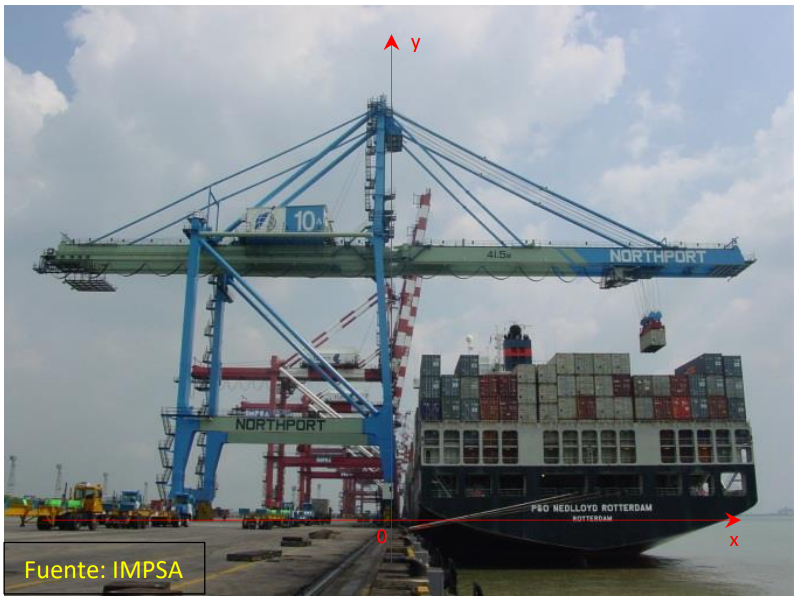
\includegraphics[width=0.85\textwidth]{images/imagen_1_sistema_ref_grua.png}
	\caption{\label{fig:ref_grua} Sistema de referencia de los ejes x e y de la grúa.}
\end{figure}

Luego si analizamos la siguiente figura \ref{fig:sistema_carro} donde se esquematiza el sistema del carro, cable de carro y sistema de transmisión. Podemos ver que el carro se mueve sobre los rieles con un movimiento de rodadura pura (rotación sin deslizamiento), y que el sistema de transmisión del carro se compone de un motor, una caja reductora, un tambor (que contiene el cable del carro) y un freno.

\begin{figure}[h!]
	\centering
	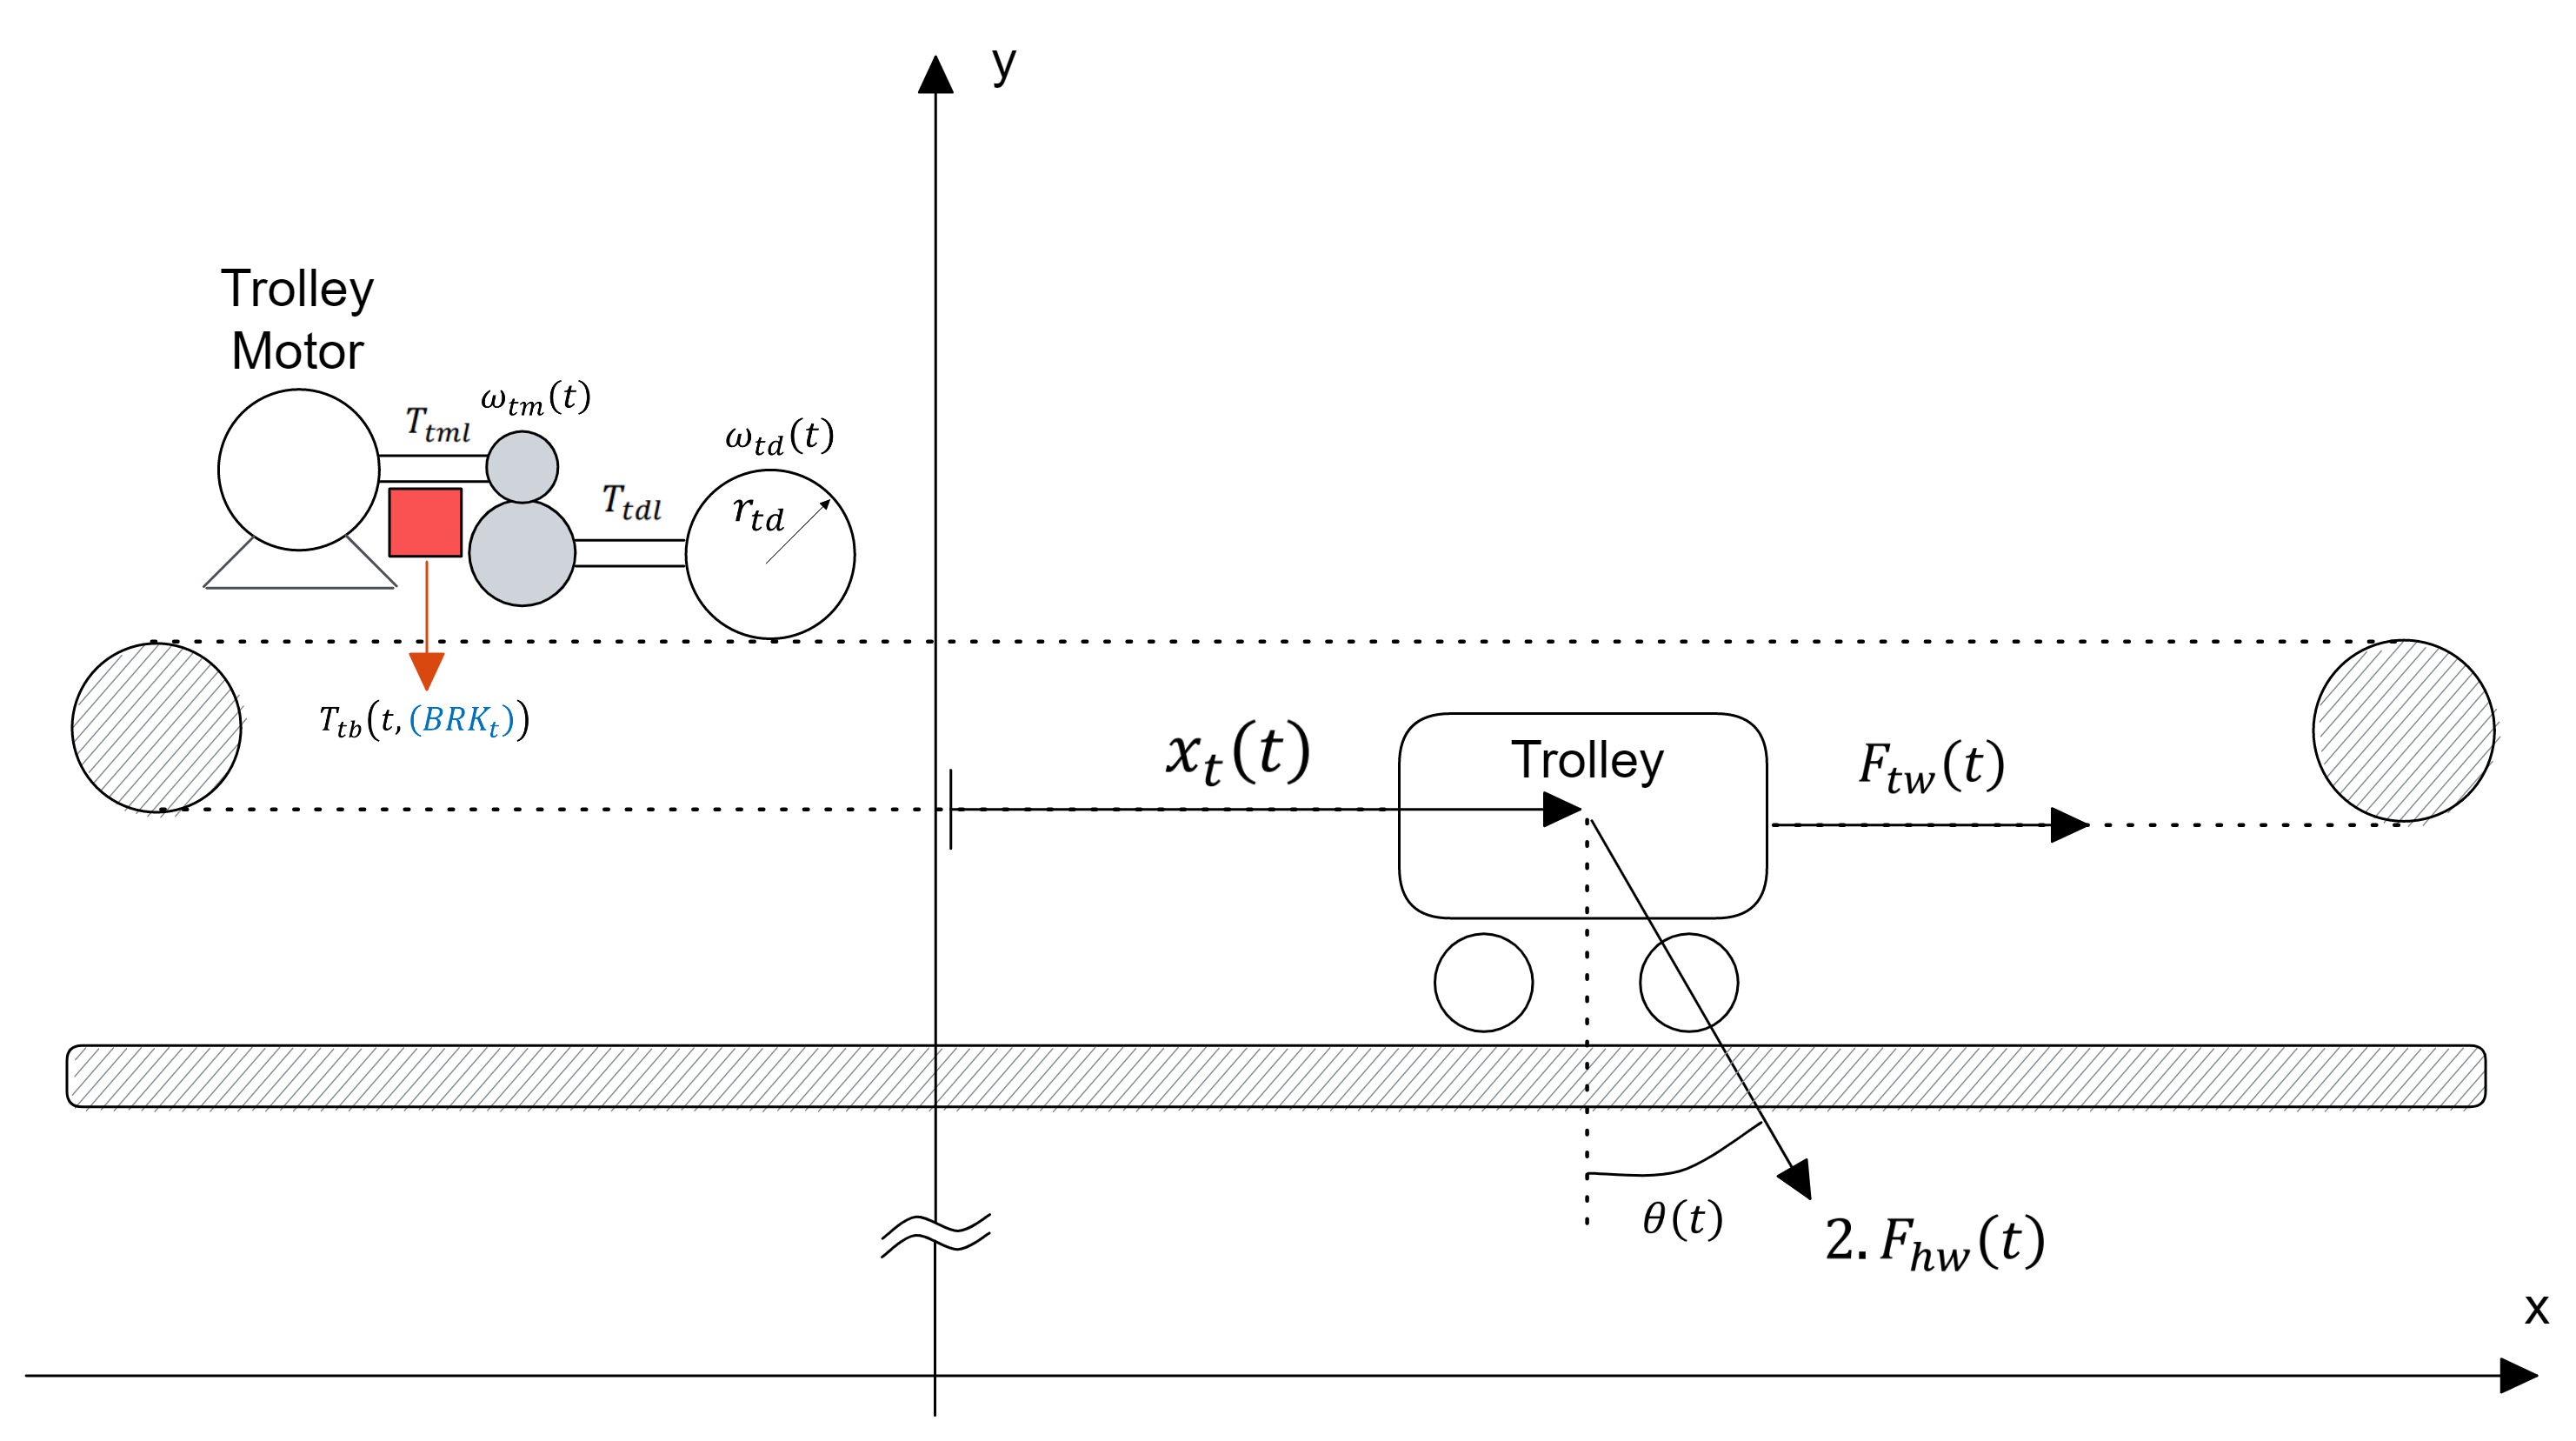
\includegraphics[width=1\textwidth]{images/imagen_2_sistema_carro.png}
	\caption{\label{fig:sistema_carro} Diseño esquemático del sistema del carro.}
\end{figure}
\newpage
A partir de esto podemos deducir la siguiente ecuación \ref{eq:sistema_carro}, que representa el movimiento del carro:
\begin{equation}
	\label{eq:sistema_carro}
	M_{t}\cdot\dot{v}_{t}(t)=F_{tw}(t)-b_{t}\cdot v_{t}(t)+2\cdot F_{hw}(t)\cdot sin(\theta(t))
\end{equation}

Donde:
\begin{itemize}
	\item $M_{t}$ es la masa equivalente del carro, ruedas, etc.
	\item $b_{t}$ es el coeficiente de fricción viscosa equivalente del carro.
	\item $x_{t}$, $v_{t}$ y $\dot{v}_{t}$ son la posición, velocidad y aceleración del carro respectivamente.
	\item $F_{tw}$ es la fuerza de tracción del cable de carro.
	\item $F_{hw}$ es la fuerza que ejerce el cable de izaje sobre el carro (por la acción de la gravedad sobre la carga).
\end{itemize}

Además la fuerza $F_{tw}$ es la que ejerce el cable de carro sobre el carro, y se puede expresar según la ecuación \ref{eq:f_tw}:
\begin{equation}
	\label{eq:f_tw}
	F_{tw}(t)=K_{tw}\left ( x_{td}(t) - x_{t}(t) \right ) + b_{tw}\left ( v_{td}(t) - v_{t}(t) \right )
\end{equation}
Donde:
\begin{itemize}
	\item $K_{tw}$ es la rigidez equivalente total a tracción del cable tensado de carro.
	\item $b_{tw}$ es la fricción interna o amortiguamiento total del cable tensado de carro.
\end{itemize}
Si tenemos en cuenta el radio primitivo del tambor $r_{td}$ y las relaciones $v_{td}(t)=r_{td}\cdot\omega_{td}(t)\ \ ;\ \ F_{tw}(t)\cdot r_{td} = T_{tdl}(t)$. Podemos expresar la ecuación \ref{eq:sistema_carro} referida al eje lento del tambor, como se muestra en la ecuación \ref{eq:sistema_carro_eje_lento}:

\begin{equation}
	\label{eq:sistema_carro_eje_lento}
	J_{td}\cdot \dot{\omega}_{td}(t)=T_{td}(t)-b_{td}\cdot\omega_{td}(t) - T_{tdl}(t)
\end{equation}

Donde:
\begin{itemize}
	\item $J_{td}$ es la inercia equivalente del eje lento (tambor y etapa de salida de la caja reductora).
	\item $b_{td}$ es el coeficiente de fricción viscosa equivalente del eje lento.
	\item $T_{td}$ es el torque de tracción del motor sobre el eje lento (a través de la caja reductora).
	\item $T_{tdl}$ es el torque que ejerce el cable de carro sobre el tambor del eje lento.
\end{itemize}

Y teniendo en cuenta la relación de transmisión entre el motor y el tambor, $i_{t}$, y también las siguientes relaciones $\omega_{td}(t)\cdot i_{t} = \omega_{tm}(t) \ \ ;\ \ T_{td}(t)=i_{t}\cdot T_{tml}(t)$ . Podemos expresar la ecuación \ref{eq:sistema_carro_eje_lento} referida al eje rápido del motor, como se muestra en la ecuación \ref{eq:sistema_carro_eje_rapido}:

\begin{equation}
	\label{eq:sistema_carro_eje_rapido}
	J_{tm+tb}\cdot\dot{\omega}_{tm}(t)=T_{tm}(t)+T_{tb}(t,{\color{blue}BRK_{t}})-b_{tm}\cdot\omega_{tm}(t)-T_{tml}(t)
\end{equation}

Donde:
\begin{itemize}
	\item $J_{tm+tb}$ es el momento de inercia equivalente del eje rápido (motor, disco de freno de operación y etapa de entrada de la caja reductora).
	\item $b_{tm}$ es el coeficiente de fricción viscosa equivalente del eje rápido.
	\item $T_{tb}$ es el torque del freno sobre el eje rápido.
	\item $T_{tm}$ es el torque que ejerce el motor sobre el eje rápido.
	\item $T_{tml}$ es el torque que ejerce la etapa de salida de la transmisión sobre el eje rápido.
\end{itemize}

Si tenemos en cuenta las ecuaciones \ref{eq:sistema_carro}, \ref{eq:sistema_carro_eje_lento} y \ref{eq:sistema_carro_eje_rapido}. Y las reemplazamos y operamos algebraicamente, podemos obtener la ecuación \ref{eq:sistema_carro_final} que representa el movimiento del carro:

\begin{equation}
	\label{eq:sistema_carro_final}
	\begin{matrix}
		M_{t}\cdot\dot{v}_{t}(t)=\frac{T_{tm}(t)\cdot i_{t}}{r_{td}}+\frac{T_{tb}(t,{\color{blue}BRK_{t}})\cdot i_{t}}{r_{td}}-\frac{\left ( b_{td}+b_{tm}\cdot{i_{t}}^{2} \right )}{{r_{td}}^{2}}\cdot v_{td}-\frac{\left ( J_{td}+J_{tm+tb}\cdot{i_{t}}^{2} \right )}{{r_{td}}^{2}}\cdot \dot{v}_{td}\ \ ...
		\\
		\\
		...\ \ -b_{t}\cdot v_{t}+2\cdot F_{hw}(t) \cdot sin \left ( \theta(t) \right )
	\end{matrix}
\end{equation}

En base a las ecuaciones \ref{eq:sistema_carro_final} y \ref{eq:f_tw} el diagrama de bloques en Simulink del modelo del carro queda como se aprecia en la siguiente figura \ref{fig:sistema_carro_simulink}:

\begin{figure}[h!]
	\centering
	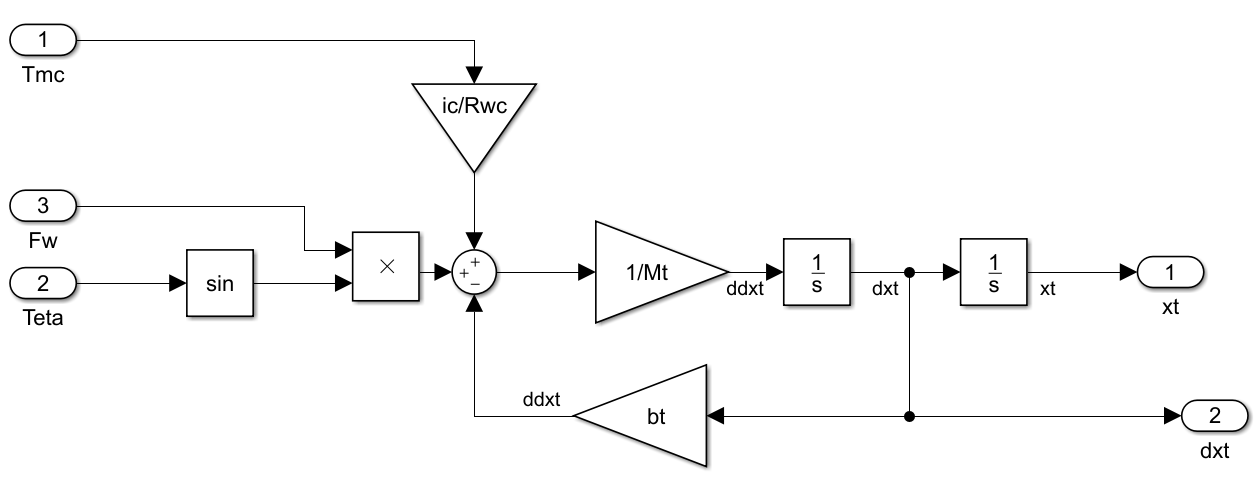
\includegraphics[width=1\textwidth]{images/imagen_3_simulink_carro.png}
	\caption{Diagrama de bloques (Simulink) del modelo del carro.}
	\label{fig:sistema_carro_simulink}
\end{figure}

\newpage

\subsection{Sistema de izaje de la carga}
\label{section:izaje}

Para el modelado del sistema de izaje tenemos que considerar las limitaciones que detallaremos a continuación:
\begin{itemize}
	\item La posición en $y_{h}\equiv Y_{t0}-l_{h}$ varía desde $-20.0\ m$ (dentro del barco) hasta $+40.0\ m$ (sobre el barco/muelle).
	\item La altura del carro y del sistema de izaje es $Y_{t0}= +45.0\ m$
	\item El despeje mínimo sobre el borde del muelle (sill beam) es $Y_{sb}= +15.0\ m$
	\item Velocidad máxima $v_{h}$: $\pm 1.5\ m/s$ (con carga nominal); $\pm 3.0\ m/s$ (sin carga). Esto es para mantenerse dentro de la curva de potencia constante durante el izaje. Ver figura \ref{fig:curva_potencia_motor}.
	\item Aceleración máxima $\dot{v}_{h}$: $\pm 0.75\ m/s^{2}$ cargado o sin carga.
\end{itemize}

\begin{figure}[h!]
	\centering
	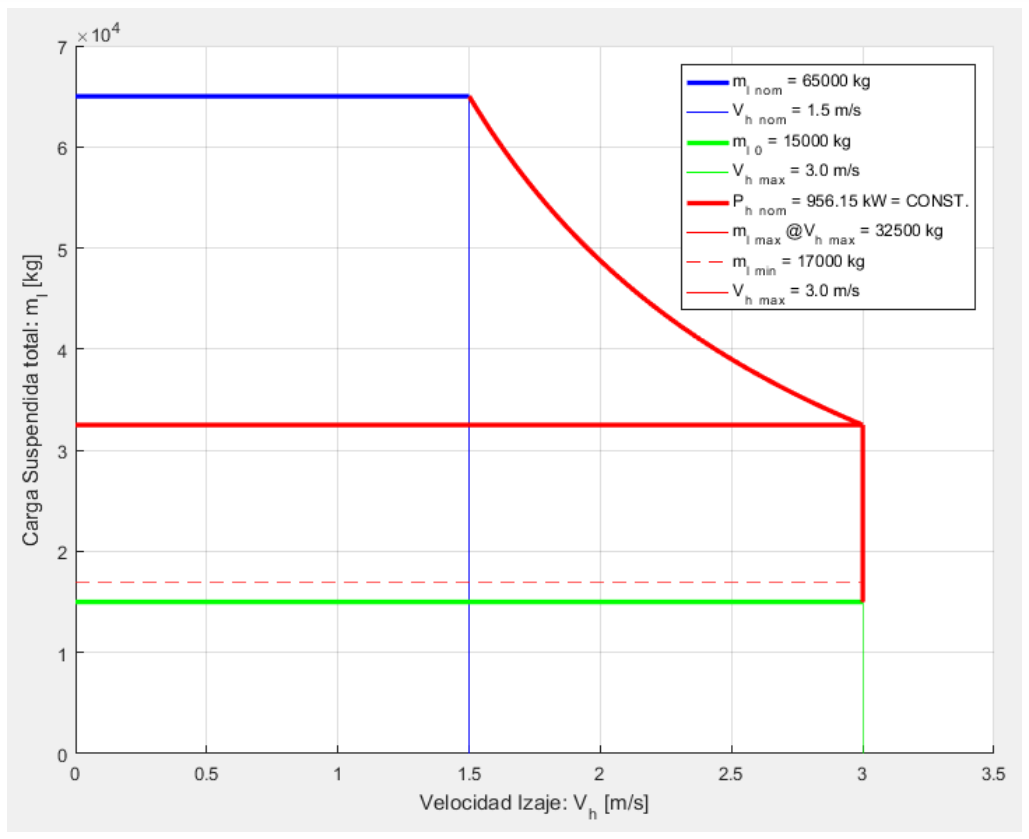
\includegraphics[width=0.7\textwidth]{images/imagen_4_curva_pot_cte.png}
	\caption{Característica de Potencia Constante - Carga suspendida vs. velocidad izaje.}
	\label{fig:curva_potencia_motor}
\end{figure}

\newpage

En base a dichas especificaciones y según la siguiente figura \ref{fig:sistema_izaje} que muestra el modelo físico del sistema de izaje.

\begin{figure}[h!]
	\centering
	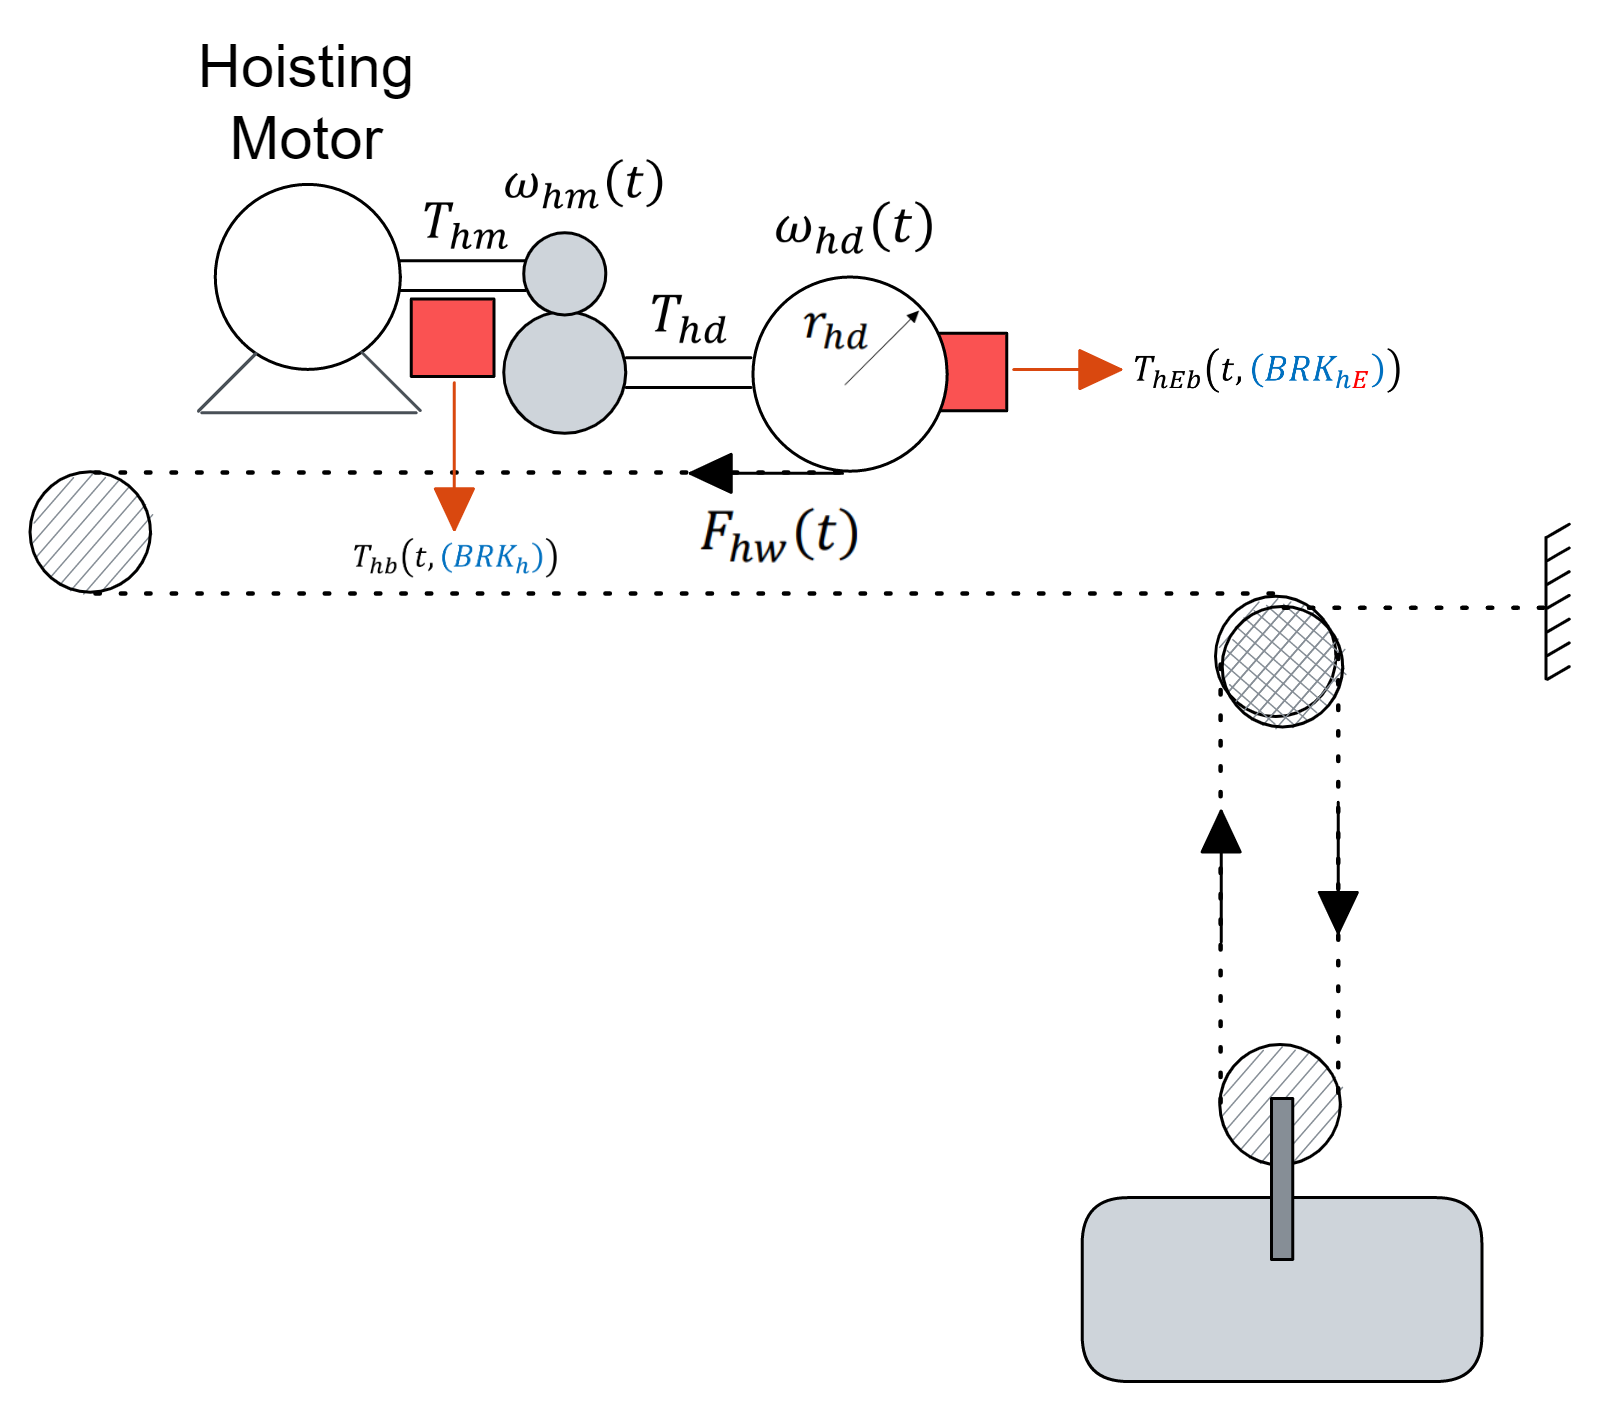
\includegraphics[width=0.85\textwidth]{images/imagen_5_sistema_izaje.png}
	\caption{Diseño esquemático del sistema de izaje y frenos.}
	\label{fig:sistema_izaje}
\end{figure}

Si aplicamos la segunda ley de newton para sistemas rotacionales, se obtiene la siguiente ecuación para el eje del motor (eje rápido):

\begin{equation}
	\label{eq:sistema_izaje_eje_rapido}
	J_{hm+hb}\cdot\dot{\omega}_{hm}(t)=T_{hm}(t)+T_{hb}(t,{\color{blue}BRK_{h}})-b_{hm}\cdot\omega_{hm}(t)-T_{hml}(t)
\end{equation}

Donde:

\begin{itemize}
	\item $J_{hm+hb}$ es el momento de inercia equivalente del eje rápido (motor, disco de freno de operación y etapa de entrada de la caja reductora).
	\item $b_{hm}$ es el coeficiente de fricción viscosa equivalente del eje rápido.
	\item $T_{hm}$ es el torque que ejerce el motor sobre el eje rápido. Torque de motorización o frenado regenerativo.
	\item $T_{hb}$ es el torque que ejerce el disco de freno de operación sobre el eje rápido.
	\item $T_{hml}$ es el torque que ejerce la etapa de salida de la transmisión y las cargas referidas al eje rápido.
\end{itemize}

De forma equivalente, podemos plantear el modelo referido al eje del tambor (eje lento). Teniendo en cuenta que $i_{h}$ es la relación de reducción entre el eje rápido y el eje lento, podemos decir que $\omega_{hd}\cdot i_{h}=\omega_{hm}$ y que $T_{hd}=i_{h}\cdot T_{hml}$.
Así obtenemos la siguiente ecuación \ref{eq:sistema_izaje_eje_lento}:

\begin{equation}
	\label{eq:sistema_izaje_eje_lento}
	J_{hd+hEb}\cdot\dot{\omega}_{hd}(t)=T_{hd}(t)+T_{hEb}(t,{\color{blue}BRK_{hE}})-b_{hd}\cdot\omega_{hd}(t)-T_{hdl}(t)
\end{equation}

Donde:

\begin{itemize}
	\item $J_{hd+hEb}$ es el momento de inercia equivalente del eje lento (tambor, disco de freno de emergencia y etapa de salida de la caja reductora).
	\item $b_{hd}$ es el coeficiente de fricción viscosa equivalente del eje lento.
	\item $T_{hd}$ es el torque que mueve el tambor, referido al eje lento.
	\item $T_{hEb}$ es el torque que ejerce el disco de freno de emergencia sobre el eje lento.
	\item $T_{hdl}$ es el torque de carga referido al eje lento.
\end{itemize}

Además considerando la siguiente ecuación \ref{eq:sistema_izaje_lh} que relaciona la posición ideal que tendría el extremo $x_{h}(t)$ en función de la longitud de cable desenrollada $l_{h}(t)$:

\begin{equation}
	\label{eq:sistema_izaje_lh}
	Y_{t0}-l_{h}(t)\equiv x_{h}(t) \Rightarrow -\dot{l_{h}}(t)=\dot{x}_{h}(t)\equiv v_{h}(t)
\end{equation}

Y teniendo en cuenta el radio primitivo del tambor de izaje $r_{hd}$, podemos decir que:

\begin{equation}
	\label{eq:sistema_izaje_vh}
	2\cdot v_{h}(t)=r_{hd}\cdot \omega_{hd}(t)\ \ \ ;\ \ \ F_{hw}(t)\cdot r_{hd}=T_{hdl}(t)
\end{equation}

Si operamos algebraicamente con las ecuaciones \ref{eq:sistema_izaje_eje_rapido}, \ref{eq:sistema_izaje_eje_lento}, \ref{eq:sistema_izaje_lh} y \ref{eq:sistema_izaje_vh}. Reemplazando y reordenando términos podemos llegar a la siguiente ecuación \ref{eq:sistema_izaje_final}:

\begin{equation}
	\label{eq:sistema_izaje_final}
	\begin{matrix}
		2\left ( \frac{{i_{h}}^{2}J_{hm+hb}+J_{hd+hEb}}{{r_{hd}}^{2}} \right )\ddot{l}_{h}=-\frac{i_{h}\left ( T_{hm}(t)+T_{hb}(t,{\color{blue}BRK_{h}}) \right )+T_{hEb}(t,{\color{blue}BRK_{hE}})}{r_{hd}}\ \ ...
		\\
		\\
		...\ \ -2\left ( \frac{{i_{h}}^{2}b_{hm}+b_{hd}}{{r_{hd}}^{2}} \right )\dot{l}_{h}+F_{hw}
	\end{matrix}
\end{equation}

En base a esta ecuación \ref{eq:sistema_izaje_final} el sistema del izaje en Simulink queda como se aprecia en la siguiente figura \ref{fig:sistema_izaje_simulink}:

\begin{figure}[h!]
	\centering
	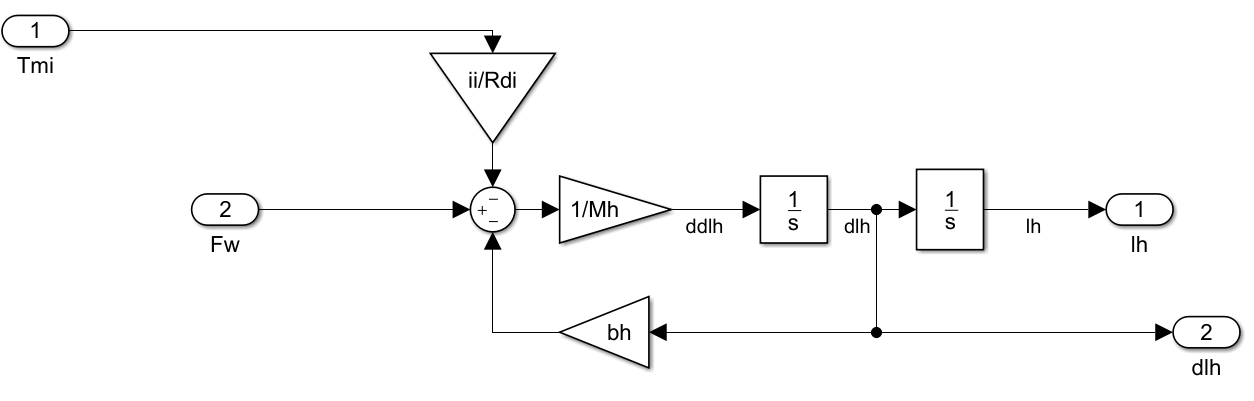
\includegraphics[width=0.7\textwidth]{images/imagen_6_simulink_izaje.png}
	\caption{Diagrama de bloques (Simulink) del modelo del izaje.}
	\label{fig:sistema_izaje_simulink}
\end{figure}

\newpage

\subsection{Análisis de tipos de carga y movimiento tipo péndulo}
\label{section:carga}

Previamente vimos que en la ecuación \ref{eq:sistema_izaje_final}, hay un término $F_{hw}(t)$ que representa la fuerza que experimenta el cable. El sistema de izaje está formado por 4 cables (1 por cada esquina del headblock) pero vamos a considerarlo como uno sólo con un modelo equivalente elástico-amortiguado dado por la siguiente ecuación \ref{eq:sistema_izaje_fuerza_cable}:

\begin{equation}
	\label{eq:sistema_izaje_fuerza_cable}
	\left\{
		\begin{matrix*}[l]
		F_{hw}(t)=2\cdot K_{w}\left ( l_{h}(t) \right )\cdot \left ( l(t)-l_{h}(t) \right )+2\cdot b_{w}\left ( l_{h}(t) \right )\cdot ( \dot{l}(t)-\dot{l_{h}}(t) ) \ \ \Leftrightarrow\ \ l(t)\geq l_{h}(t)
		\\
		\\ 
		F_{hw}(t)= 0\ \ \Leftrightarrow\ \ l(t)<l_{h}(t)
		\end{matrix*}
	\right.
\end{equation}

Donde:

\begin{equation}
	\label{eq:sistema_izaje_fuerza_cable_params}
	K_{w}\left ( l_{h}(t) \right )=\frac{K_{wu}}{2\cdot l_{h}(t)+110\ m}\ \ \ ;\ \ \ b_{w}\left ( l_{h}(t) \right )=b_{wu}\cdot \left ( 2\cdot l_{h}(t)+110\ m \right )
\end{equation}

Si tenemos en cuenta el tipo de carga al que puede estar sometido el cable, podemos tener en consideración 3 casos con diferentes límites. Los mismos son:

\begin{itemize}
	\item \textbf{Vacío:} sólo se considera la masa de Spreader + Headblock (sin container). $m_{l0}=15000\ Kg$
	\item \textbf{Carga suspendida:} esto es la masa $m_{l0}$ más el peso del contenedor. La masa total varía según el peso del contenedor entre:
		\subitem \textbf{Máxima o nominal:} $m_{l}=65000\ Kg$.
		\subitem \textbf{Mínima:} Con contenedor vacío de $2000\ Kg$. Masa total $m_{min}=17000\ Kg$.
		\subitem \textbf{Intermedio:} Es un estado intermedio entre los anteriores $m_{min}<m_{x}<m_{max}$.
	\item \textbf{Carga apoyada:} Este es un caso particular que representa el estado de operación con carga no suspendida.
	
\end{itemize}

Algo más a tener en cuenta es que cuando la carga está apoyada hay una reacción de vínculo elástico (sin deformación plástica), entre la carga y el suelo. Osea hay una compresión debido a la gravedad $g=9.80665\ \frac{m}{s^{2}}$. Para modelar este comportamiento se consideraron los siguientes parámetros:
\begin{itemize}
	\item Rigidez y coeficiente de fricción vertical (compresión): $K_{cy}=1.8\cdot 10^{9}\ \frac{N}{m}$ y $b_{cy}=1.0\cdot 10^{7}\ \frac{N}{m/s}$
	\item Coeficiente de fricción horizontal (arrastre): $b_{cx}=1.0\cdot 10^{6}\ \frac{N}{m/s}$
\end{itemize}

\subsubsection{Análisis con carga suspendida}

Con lo visto previamente ya sabemos que, el cable equivalente no soporta compresión. Ya que en tal caso se doblaría. Por ende, si se denomina $l(t)$ a la longitud real del cable fuera del tambor (estirado) y $l_{h}(t)$ a la longitud del cable desenrollado sin estar sometido a ninguna fuerza.

Y considerando pequeñas deformaciones, dentro del límite elástico. Es válida la Ley de Hooke para sistemas amortiguados. Es decir, que la fuerza que experimenta el cable es proporcional a la deformación del mismo según la ecuación \ref{eq:sistema_izaje_fuerza_cable}.

Entonces, si analizamos la siguiente imagen \ref{fig:sistema_pendulo} podemos ver que la longitud del cable $l(t)$ es mayor que la longitud del cable desenrollado $l_{h}(t)$ cuando la carga está suspendida. Por lo tanto, la fuerza que experimenta el cable es positiva y el sistema de izaje se estira. En el caso contrario, la fuerza del cable es nula.

\begin{figure}[h!]
	\centering
	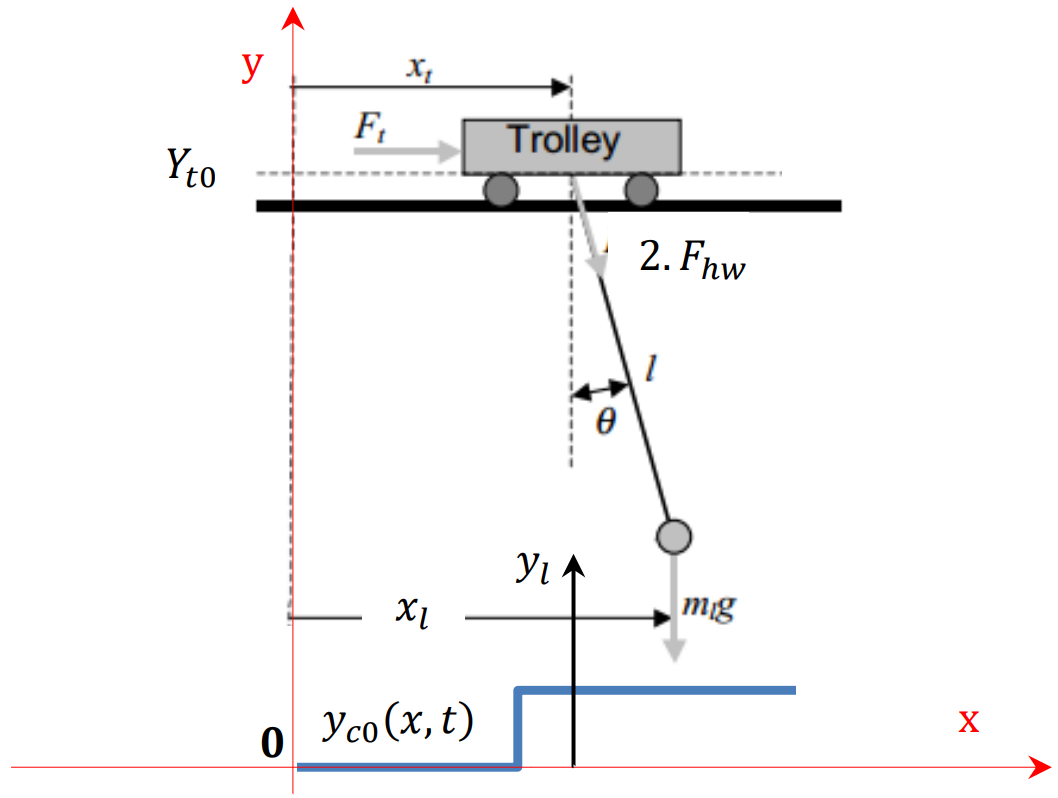
\includegraphics[width=0.7\textwidth]{images/imagen_7_sistema_pendulo.png}
	\caption{Sistema de izaje con carga suspendida.}
	\label{fig:sistema_pendulo}
\end{figure}

\newpage

En base a este modelo podemos plantear la siguiente ecuación \ref{eq:sistema_pendulo_cinematica} que representa el sistema de un péndulo y un cambio de coordenadas globales a locales de movimiento.

\begin{equation}
	\label{eq:sistema_pendulo_cinematica}
	\left\{
		\begin{matrix*}[l]
		x_{l}(t)=x_{t}(t) + l(t)\cdot \sin(\theta(t))
		\\
		\\ 
		y_{l}(t)=Y_{t0} - l(t)\cdot \cos(\theta(t))
		\end{matrix*}
	\right.
\end{equation}

Dicha ecuación también se puede expresar como:

\begin{equation}
	\label{eq:sistema_pendulo_cinematica_raiz_tangente}
	\left\{
		\begin{matrix*}[l]
		l(t)=\sqrt{\left ( x_{l}(t)-x_{t}(t) \right )^{2}+\left ( Y_{t0}-y_{l}(t) \right )^{2}}
		\\
		\\ 
		\theta(t)=\arctan \left ( \frac{x_{l}(t)-x_{t}(t)}{Y_{t0}-y_{l}(t)} \right )
		\end{matrix*}
	\right.
\end{equation}

Y cuyo gráfico se muestra en la figura \ref{fig:sistema_pendulo_cinematica_raiz_tangente}.

\begin{figure}[h!]
	\centering
	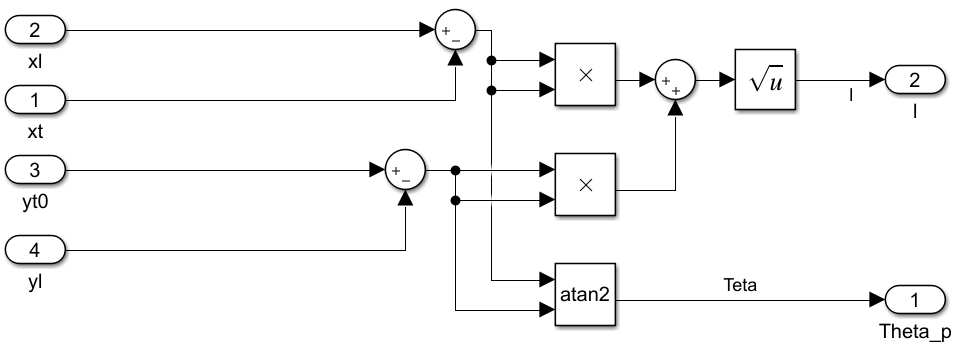
\includegraphics[width=0.7\textwidth]{images/imagen_8_sistema_pendulo_cinematica_raiz_tangente.png}
	\caption{Gráfico de la ecuación \ref{eq:sistema_pendulo_cinematica_raiz_tangente}.}
	\label{fig:sistema_pendulo_cinematica_raiz_tangente}
\end{figure}

\newpage

La dinámica del sistema se puede expresar como la siguiente ecuación \ref{eq:sistema_pendulo_dinamica_carga_suspendida}, sólo para carga suspendida donde $y_{l}(t)-h_{c}({\color{blue}TLK})>y_{c0}(x,y)$:

\begin{equation}
	\label{eq:sistema_pendulo_dinamica_carga_suspendida}
	\left\{
		\begin{matrix*}[l]
		m_{l}({\color{blue}TLK})\cdot \dot{v}_{xl}(t)= -2 \cdot F_{hw}(t)\cdot \sin(\theta(t))
		\\
		\\ 
		m_{l}({\color{blue}TLK})\cdot \dot{v}_{yl}(t)=2 \cdot F_{hw}(t)\cdot \cos(\theta(t))-m_{l}({\color{blue}TLK})\cdot g
		\end{matrix*}
	\right.
\end{equation}

\subsubsection{Análisis con carga apoyada}

Si en cambio no encontramos en la condición de la carga apoyada, es decir, $y_{l}(t)-h_{c}({\color{blue}TLK})\geq y_{c0}(x,y)$, entonces la ecuación \ref{eq:sistema_pendulo_dinamica_carga_suspendida} queda como la siguiente ecuación \ref{eq:sistema_pendulo_dinamica_carga_apoyada}:

\begin{equation}
	\label{eq:sistema_pendulo_dinamica_carga_apoyada}
	\left\{
		\begin{matrix*}[l]
		m_{l}({\color{blue}TLK})\cdot \dot{v}_{xl}(t)= -2 \cdot F_{hw}(t)\cdot \sin(\theta(t))-b_{cx}\cdot v_{xl}(t)
		\\
		\\ 
		m_{l}({\color{blue}TLK})\cdot \dot{v}_{yl}(t)=2 \cdot F_{hw}(t)\cdot \cos(\theta(t))-m_{l}({\color{blue}TLK})\cdot g + K_{cy} \left ( y_{c0}(x,t)-y_{l}(t)+h_{c}({\color{blue}TLK}) \right )-b_{cy}\cdot v_{yl}(t)
		\end{matrix*}
	\right.
\end{equation}

De esta forma, obtenemos que el diagrama que representa las ecuaciones \ref{eq:sistema_pendulo_dinamica_carga_suspendida}, \ref{eq:sistema_pendulo_dinamica_carga_apoyada}, \ref{eq:sistema_izaje_fuerza_cable} y \ref{eq:sistema_izaje_fuerza_cable_params} es el siguiente:

\begin{figure}[h!]
	\centering
	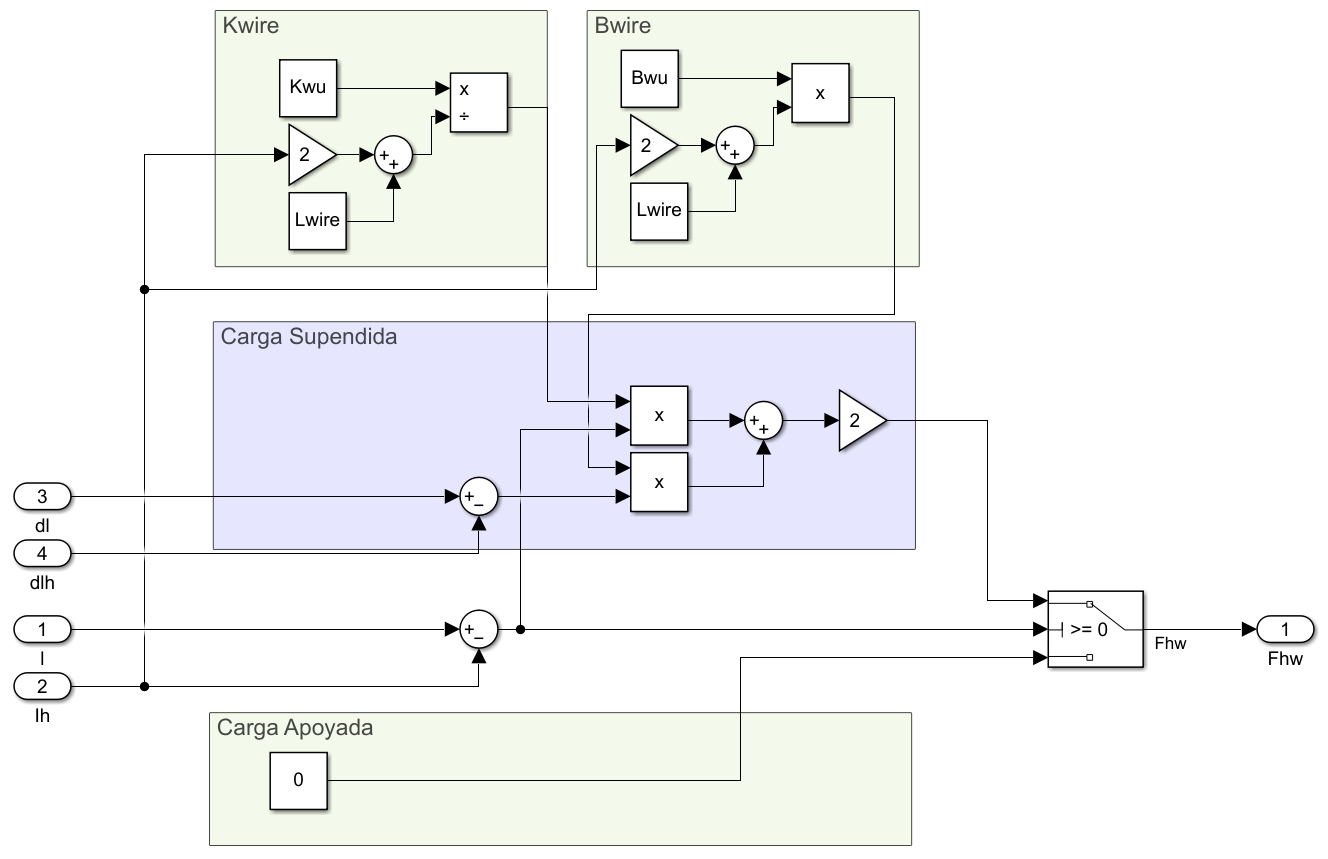
\includegraphics[width=1\textwidth]{images/imagen_9_sistema_pendulo_dinamica.png}
	\caption{Diagrama de la dinámica del sistema.}
	\label{fig:sistema_pendulo_dinamica}
\end{figure}

Donde si además consideramos las ecuaciones \ref{eq:sistema_pendulo_cinematica} y \ref{eq:sistema_pendulo_cinematica_raiz_tangente}, obtenemos el siguiente diagrama:

\begin{figure}[h!]
	\centering
	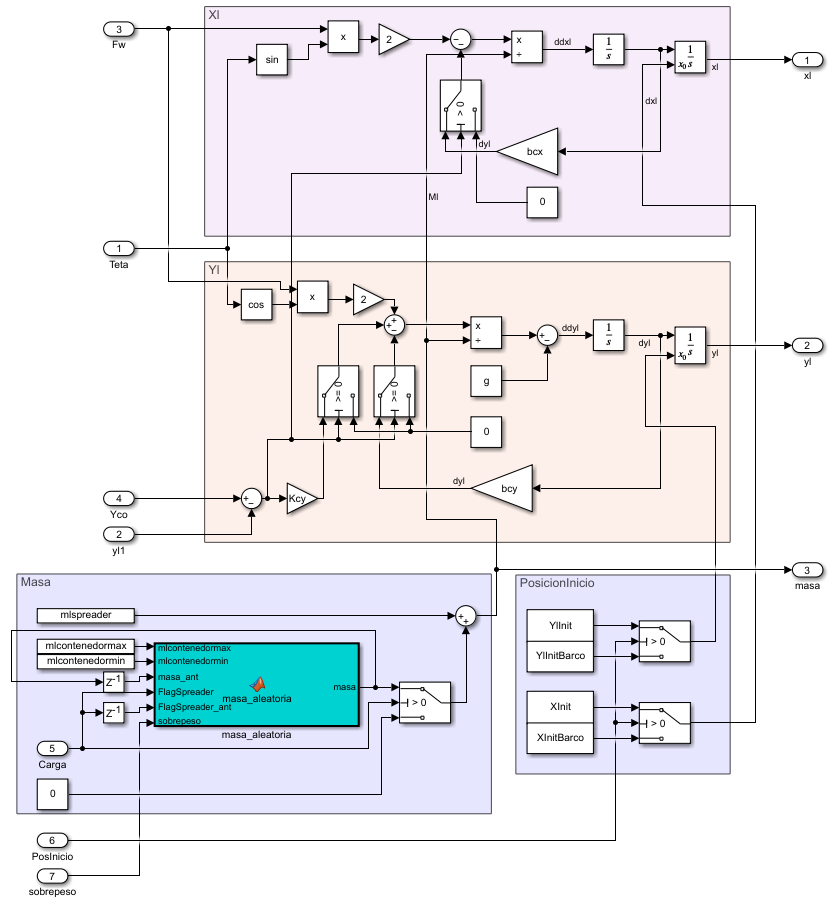
\includegraphics[width=1\textwidth]{images/imagen_10_sistema_pendulo_cinematica_dinamica.png}
	\caption{Diagrama en Simulink del modelo completo del pendulo.}
	\label{fig:sistema_pendulo_cinematica_dinamica}
\end{figure}

\newpage

Llegados a este punto, procedemos a unir los siguientes modelos físicos dando lugar al modelo de la planta que se muestra en la figura \ref{fig:sistema_completo}.
\begin{itemize}
	\item Carro \ref{section:carro}
	\item Izaje \ref{section:izaje}
	\item Carga \ref{section:carga}
\end{itemize}

\begin{figure}[h!]
	\centering
	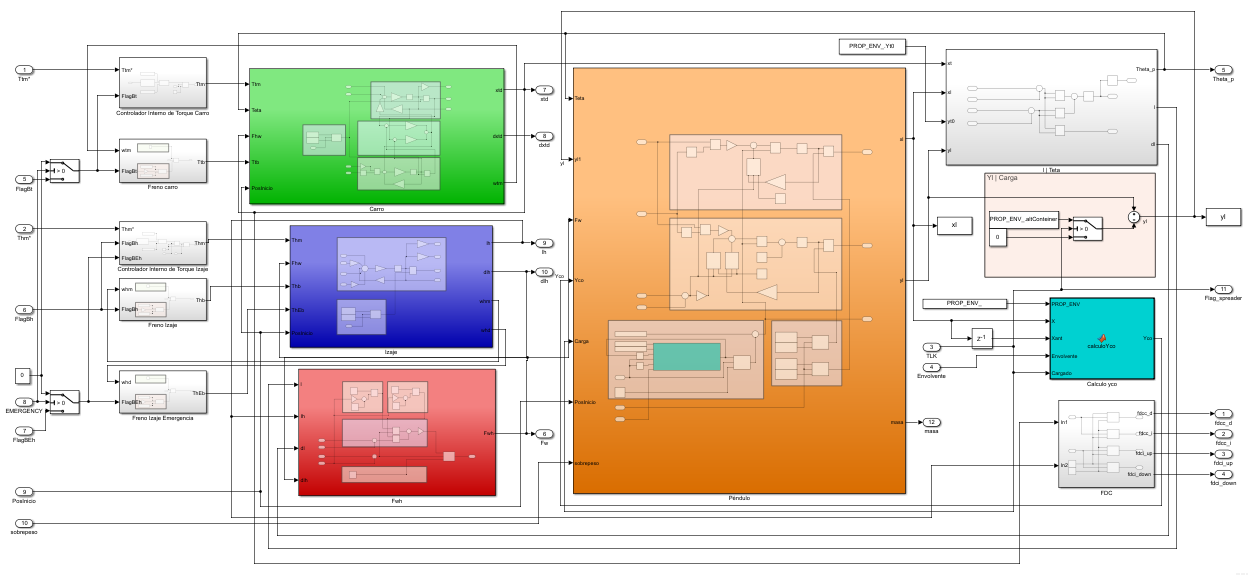
\includegraphics[width=1\textwidth]{images/imagen_11_sistema_completo.png}
	\caption{Diagrama en Simulink del modelo completo del pendulo.}
	\label{fig:sistema_completo}
\end{figure}

% \subsection{Modos de freno mecánico}

% \subsection{Controladores internos de torque}

\section{Sistemas de control}

Tal como se explicó anteriormente, el sistema físico a controlar consta de 2 movimientos principales: el de traslación del carro (horizontal, eje $x$) y el de izaje de la carga (vertical, eje $y$). Hay que tener en cuenta que ambos movimientos están acoplados ya que el sistema de izaje se desplaza junto con el movimiento del carro. Y además la carga (spreader + contenedor) se balancea, suspendida del carro que la sube/baja mediante los cables de izaje. Para poder controlar de forma eficiente estos movimientos se consideran los siguientes niveles de control para un autómata híbrido de control:

\begin{itemize}
	\item \textbf{Nivel 0:} Este es el control de seguridad que consiste en un autómata reducido y confiable, que es el encargado de actuar o accionar ante una falla crítica de niveles inferiores y/o riesgo del sistema físico o de seguridad (colisiones).
	\item \textbf{Nivel 1:} Este es el control supervisor global y es un control de estados discretos activados por eventos, con estructura jerárquica y concurrencia, para una operación suave y eficiente con coordinación y optimización de trayectorias, es un control de operación global del sistema.
	\item \textbf{Nivel 2:} Acá se encuentran los controladores de movimiento de estados continuos en tiempo discreto. Son los que reciben las consignas de movimiento individuales del control supervisor para el control de cada uno de los movimientos principales.
\end{itemize}

\subsection{Nivel 2 - Controladores de movimiento}
Los controladores de este nivel son del tipo PID para los movimientos de traslación del carro y de izaje de la carga, y además se tiene en cuenta un controlador PD para el modelo de balanceo de la carga.

Para cada uno de estos plantearemos sus transformadas de Laplace para luego obtener las funciones de transferencia de cada sistema. Una vez conocidas dichas funciones de transferencia, se procederá a obtener los polos y ceros del sistema, para así poder obtener los parámetros óptimos de los controladores PID por método de sintonía serie.

\newpage

\subsubsection{Controlador de posición del carro}
Recordando la ecuación \ref{eq:sistema_carro_final}, ecuación final que modela el movimiento del carro, si la expresamos en función de su velocidad. Sin considerar los torques de freno y teniendo en cuenta la simplificación $v_{td}(t)\simeq v_{t}(t)$ obtenemos la siguiente ecuación \ref{eq:sistema_carro_simplificado}:

\begin{equation}
	\label{eq:sistema_carro_simplificado}
	\left ( M_{t}+ \frac{J_{td}+J_{tm+tb}\cdot{i_{t}}^{2}}{{r_{td}}^{2}} \right )\cdot\dot{v}_{t}(t)=\frac{T_{tm}(t)\cdot i_{t}}{r_{td}}-\left (b_{t} +\frac{b_{td}+b_{tm}\cdot{i_{t}}^{2}}{{r_{td}}^{2}} \right )\cdot v_{t} + 2\cdot F_{hw}(t) \cdot sin \left ( \theta(t) \right )
\end{equation}

Donde vamos a decir que:

\begin{equation}
	\label{eq:sistema_carro_masa_equivalente}
	M_{eqt} = \left ( M_{t}+ \frac{J_{td}+J_{tm+tb}\cdot{i_{t}}^{2}}{{r_{td}}^{2}} \right )
\end{equation}

y

\begin{equation}
	\label{eq:sistema_carro_friccion_equivalente}
	b_{eqt} = b_{t} +\frac{b_{td}+b_{tm}\cdot{i_{t}}^{2}}{{r_{td}}^{2}}
\end{equation}

Así podemos reescribir la ecuación \ref{eq:sistema_carro_simplificado} como:

\begin{equation}
	\label{eq:sistema_carro_simplificado_params_equivalentes}
	M_{eqt}\cdot\dot{v}_{t}(t)=\frac{T_{tm}(t)\cdot i_{t}}{r_{td}}-b_{eqt}\cdot v_{t} + 2\cdot F_{hw}(t) \cdot sin \left ( \theta(t) \right )
\end{equation}

Con esto ahora podemos decir que la ecuación \ref{eq:sistema_carro_simplificado_params_equivalentes}, aplicando tansformada de Laplace. Y aplicando el cambio de $F_{l}(s)=F_{hw}(s) \cdot sin \left ( \theta(s) \right )$ se puede escribir como:

\begin{equation}
	\label{eq:sistema_carro_simplificado_laplace}
	M_{eqt}\cdot s\cdot V_{t}(s) = \frac{T_{tm}(s)\cdot i_{t}}{r_{td}}-b_{eqt}\cdot V_{t}(s) + 2\cdot F_{l}(s)
\end{equation}

Reordenando la ecuación \ref{eq:sistema_carro_simplificado_laplace} obtenemos:

\begin{equation}
	\label{eq:sistema_carro_simplificado_laplace_reordenado}
	\left ( M_{eqt}\cdot s+b_{eqt} \right )\cdot V_{t}(s) = \frac{T_{tm}(s)\cdot i_{t}}{r_{td}}+ 2\cdot F_{l}(s)
\end{equation}

Donde $V_{t}(t)$ es la velocidad del carro. Y como se puede apreciar en la ecuación \ref{eq:sistema_carro_simplificado_laplace_reordenado} se tienen 3 entradas del sistema: el torque del motor del carro $T_{tm}(s)$, el torque del freno de operación del carro $T_{tb}$ y la fuerza que ejerce la carga sobre el carro $2\cdot F_{l}(s)$. Así, se tiene una función de transferencia para cada una de ellas:

\begin{equation}
	\label{eq:sistema_carro_simplificado_laplace_G1t}
	G_{1t}(s)=\frac{V_{t}(s)}{T_{tm}(s)}=\frac{i_{t}}{r_{td}\cdot (M_{eqt}\cdot s+b_{eqt})}
\end{equation}

\begin{equation}
	\label{eq:sistema_carro_simplificado_laplace_G2t}
	G_{2t}(s)=\frac{V_{t}(s)}{F_{l}(s)}=\frac{2}{M_{eqt}\cdot s+b_{eqt}}
\end{equation}

Como las entradas de control son de torque, las ecuaciones de interés son $G_{1t}(s)$. Los polos de dichas ecuaciones se ubican en:

\begin{equation}
	\label{eq:sistema_carro_simplificado_laplace_polos}
	\omega_{G1t}=-\frac{b_{eqt}}{M_{eqt}}
\end{equation}

Siempre buscamos tener una respuesta del controlador óptima por lo cuál la misma debe ser más rápida que la velocidad de respuesta de la planta. Para esto aplicamos el método de sintonía serie y definimos que la frecuencia del controlador $\omega_{post}=10\cdot \omega_{G_{1t}}$ y para tener un sistema subamortiguado se adopta un factor $n_{t}=2.5$ correspondiente a un factor de amortiguamiento de $\xi =0.75$. De esa forma obtenemos con el método las siguientes ganancias del controlador:

\begin{itemize}
	\item Proporcional $\rightarrow K_{pc} = M_{eqt}\cdot n_{t}\cdot {\omega_{post}}^{2} = 1.961 \cdot 10^6$
	\item Integral $\rightarrow K_{ic} = M_{eqt}\cdot {\omega_{post}}^{3}  = 7.089 \cdot 10^6$
	\item Derivativo $\rightarrow K_{dc} = M_{eqt}\cdot n_{t}\cdot {\omega_{post}} = 5.42 \cdot 10^5$
\end{itemize}

Así llegamos a la ecuación genérica del control PID de movimiento horizontal que nos queda de la siguiente forma:

\begin{equation}
	\label{eq:sistema_carro_simplificado_laplace_controlador}
	T_{mc}^{*}(s)=G_{T}(s)\left [ K_{dc}+\frac{1}{s}\cdot K_{pc}+\frac{1}{s^{2}}\cdot K_{ic} \right ] e_{dxt}(s)
\end{equation}

Podemos observar que el error a medir es de velocidad, no de posición. Esto se debe a que el controlador planteado utiliza 2 integradores para evitar el uso de derivadores, que amplifican el ruido. El diagrama de bloques nos queda:

\begin{figure}[h!]
	\centering
	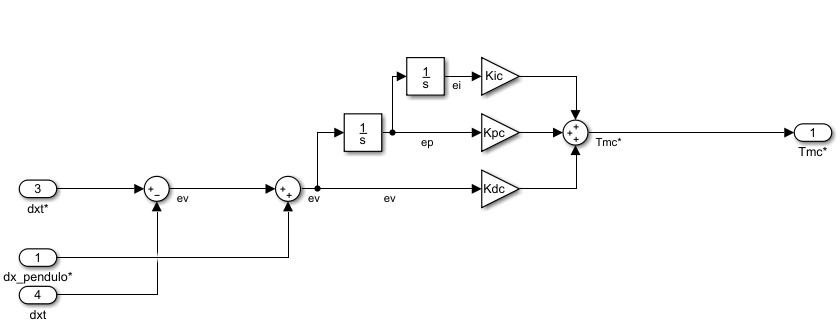
\includegraphics[width=1\textwidth]{images/imagen_12_controlador_carro.png}
	\caption{Diagrama en Simulink del controlador del carro.}
	\label{fig:controlador_carro_simulink}
\end{figure}


\subsubsection{Controlador del izaje de la carga}

Si analizamos ahora el sistema de izaje de la carga y tomamos el modelo dinámico dado por la ecuación \ref{eq:sistema_izaje_final}, sin considerar los torques de frenado. Reescribiendo $M_{eqh}$ y $b_{eqh}$ como:

\begin{equation}
	\label{eq:sistema_izaje_masa_equivalente}
	M_{eqh} = \frac{{i_{h}}^{2}J_{hm+hb}+J_{hd+hEb}}{{r_{hd}}^{2}}
\end{equation}

\begin{equation}
	\label{eq:sistema_izaje_friccion_equivalente}
	b_{eqh} = \frac{{i_{h}}^{2}b_{hm}+b_{hd}}{{r_{hd}}^{2}}
\end{equation}

Así despejando la ecuación \ref{eq:sistema_izaje_final} junto con las que acabamos de mencionar. Expresandolas en función de su velocidad (para evitar usar un derivador) y si tratamos a la fuerza de la carga como una perturbación del sistema. Podemos aplicar transformada de Laplace y obtener las siguientes ecuaciones:

\begin{equation}
	\label{eq:sistema_izaje_simplificado_laplace}
	2\cdot s\ M_{eqh} V_{lh}(s)=-\frac{ T_{hm}(s)\cdot i_{h}}{r_{hd}}-2\ b_{eqh} V_{lh}(s)+F_{hw}(s)
\end{equation}

Reagrupando:
\begin{equation}
	\label{eq:sistema_izaje_simplificado_laplace_reordenado}
	2\cdot \left ( M_{eqh}\cdot s+b_{eqh} \right )\cdot V_{lh}(s) = \frac{T_{hm}(s)\cdot i_{h}}{r_{hd}}+ F_{hw}(s)
\end{equation}

Donde $V_{lh}(t)$ representa a la velocidad del izaje. Y como podemos ver en la ecuación \ref{eq:sistema_izaje_simplificado_laplace_reordenado} se tienen 2 entradas del sistema: el torque $T_{hm}(s)$ y la tensión a la que se somete el cable $F_{hw}(s)$. Así podemos expresar las funciones de transferencia para cada entrada como:

\begin{equation}
	\label{eq:sistema_izaje_simplificado_laplace_G1h}
	G_{1h}(s)=\frac{V_{lh}(s)}{T_{hm}(s)}=\frac{i_{h}}{r_{hd}\cdot (M_{eqh}\cdot s+b_{eqh})}
\end{equation}

\begin{equation}
	\label{eq:sistema_izaje_simplificado_laplace_G2h}
	G_{2h}(s)=\frac{V_{lh}(s)}{F_{hw}(s)}=\frac{2}{M_{eqh}\cdot s+b_{eqh}}
\end{equation}

La entrada de control es de torque, por lo tanto la ecuación de interés es $G_{1h}(s)$. Que tiene un polo que está ubicado en:

\begin{equation}
	\label{eq:sistema_izaje_simplificado_laplace_polos}
	\omega_{G1h}=-\frac{b_{eqh}}{M_{eqh}}
\end{equation}

Nuevamente tenemos que asegurar que la respuesta del controlador sea más rápida que la de la planta por lo cuál aplicando el método de sintonía serie con una frecuencia del controlador de $\omega_{posh}=10\cdot \omega_{G_{1h}}$. Y para obtener un sistema subamortiguado tomaremos un factor $n_{h}=2.5$ correspondiente a un factor de amortiguamiento de $\xi =0.75$. Así obtenemos las siguientes ganancias del controlador:

\begin{itemize}
	\item Proporcional $\rightarrow K_{pi} = M_{eqh}\cdot n_{h}\cdot {\omega_{posh}}^{2} = 1.2577 \cdot 10^5$
	\item Integral $\rightarrow K_{ii} = M_{eqh}\cdot {\omega_{posh}}^{3}  = 2.3947 \cdot 10^5$
	\item Derivativo $\rightarrow K_{di} = M_{eqh}\cdot n_{h}\cdot {\omega_{posh}} = 2.6424\cdot 10^4$
\end{itemize}

Quedando entonces, la ecuación genérica del PID del izaje como:

\begin{equation}
	\label{eq:sistema_izaje_simplificado_laplace_controlador}
	T_{mi}^{*}(s)=G_{T}(s)\left [ K_{di}+\frac{1}{s}\cdot K_{pi}+\frac{1}{s^{2}}\cdot K_{ii} \right ] e_{dlh}(s)
\end{equation}

\begin{figure}[h!]
	\centering
	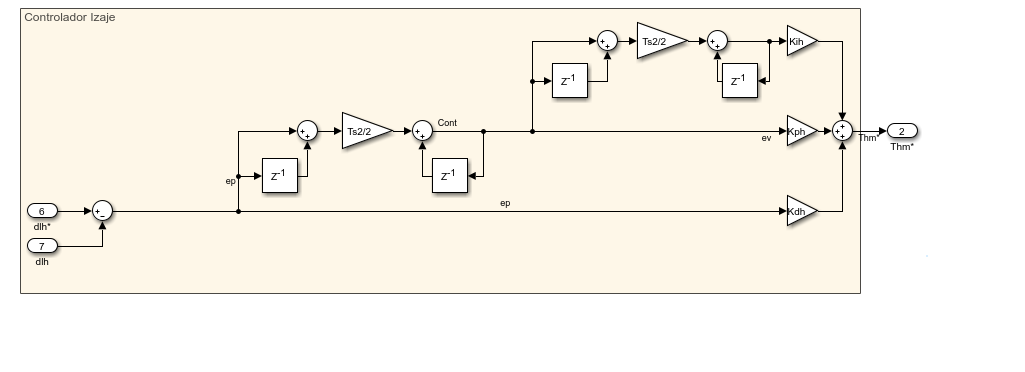
\includegraphics[width=1\textwidth]{images/imagen_13_controlador_izaje.png}
	\caption{Diagrama en Simulink del controlador de izaje.}
	\label{fig:controlador_izaje_simulink}
\end{figure}

\newpage

\subsubsection{Controlador del péndulo (ángulo de balanceo de la carga)}

Durante la operación de traslación de la carga se tienen desplazamientos no deseados como consecuencia del balanceo y la inercia que lleva la misma carga que transportamos. Por esto se incluye un control automático realimentado para controlar dicho balanceo de la carga durante la operación. Con esto esperamos amortiguar las oscilaciones en la trayectoria alrededor del punto de equilibrio dinámico. Las especificaciones de desempeño del controlador son:

\begin{itemize}
	\item Ángulo máximo aceleración/desaceleración $=\pm 20°$
	\item Ángulo máximo trayectoria a velocidad ``constante'' $=\pm 5°$
	\item Ángulo residual movimiento completado y carro detenido $=\pm 1°$
\end{itemize}

Para compensar el error de este ángulo vamos a implementar un control del tipo PD con ganancias ajustadas en función de la altura de izaje (longitud del péndulo equivalente). Vamos a partir de un sistema carro-péndulo como el que se puede apreciar en la siguiente figura \ref{fig:sistema_carro_pendulo}:

\begin{figure}[h!]
	\centering
	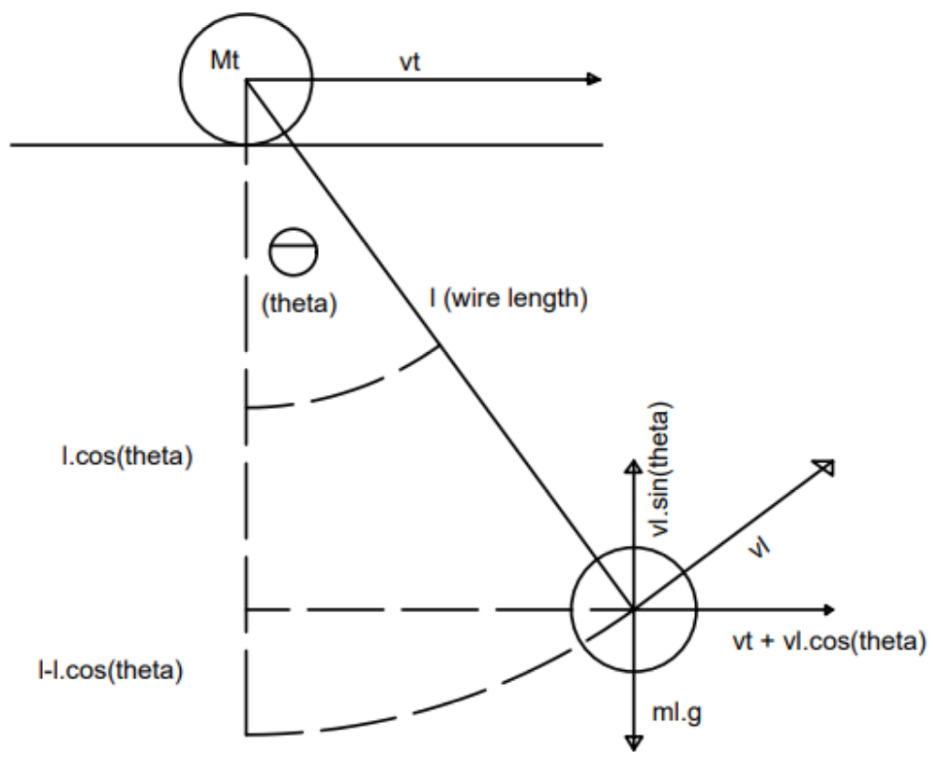
\includegraphics[width=0.7\textwidth]{images/imagen_14_sistema_carro_pendulo.png}
	\caption{Diagrama del sistema carro péndulo.}
	\label{fig:sistema_carro_pendulo}
\end{figure}

Ahora necesitamos expresar esto como ecuaciones matemáticas, por lo cuál es necesario determinar las entradas (medidas con sensores) y salidas (acciones de control) del sistema. Las mismas son:

\begin{itemize}
	\item \textbf{Entrada:} $\theta (t)$ ángulo entre la carga y el carro.
	\item \textbf{Salida:} $\dot{x}_{t}(t)$ velocidad del carro, como debería moverse para evitar el balanceo, que a su vez corresponde a la entrada del controlador PID utilizado para el movimiento horizontal.
\end{itemize}

Así procedemos a determinar la función de transferencia del sistema basados en la entrada y salida elegidas. También como se trata de un pseudo péndulo simple una forma de calcular el sistema es con un enfoque energético basado en la formulación de Lagrange. Para obtener el Lagrangiano hay que aplicar la siguiente expresión:

\begin{equation}
	\label{eq:lagrangiano}
	L(t)=K(t)-U(t)
\end{equation}

Donde, $K$ es la energía cinética del sistema, y $U$ es la energía potencial del sistema. En primer lugar, la energía cinética total del sistema está dada por la suma de la energía del carro $K_{t}$ y de la carga $K_{l}$ quedando como:

\begin{equation}
	\label{eq:lagrangiano_energia_cinetica}
	K(t)=K_{t}(t)+K_{l}(t)=\frac{1}{2}\left ( m_{t}\cdot {v_{t}}^2(t)+m_{l}\cdot {v_{l}}^2(t) \right )
\end{equation}

Donde, $v_{l}(t)$ es la velocidad de la carga. Observando la figura \ref{fig:sistema_carro_pendulo}, la masa (carga) tiene una velocidad $v_{l}(t)$ que es perpendicular al cable. Entonces podemos proceder a descomponer esta velocidad en $v_{x}(t)$ y $v_{y}(t)$ (donde $x$ es el eje horizontal e $y$ es el eje vertical), con esto vamos a poder simplificar las funciones trigonométricas. Quedando las ecuaciones como:

\begin{equation}
	\label{eq:lagrangiano_velocidades_energia_cinetica}
	\begin{matrix}v_{\theta }(t)=\dot{\theta }(t)\cdot l\ \ \ ;\ \ \ v_{t}(t)=\dot{x_{t}}(t) \\ \\ {v_{l}}^{2}(t)=\left [ \dot{x_{t}}(t)+\dot{\theta }(t)\cdot l\cdot cos\left ( \theta (t) \right ) \right ]^{2} + \left [ \dot{\theta }(t)\cdot l\cdot sin\left ( \theta (t) \right ) \right ]^{2} \\ \\ {v_{l}}^{2}(t)= {\dot{x_{t}}}^{2}(t)+2\dot{x_{t}}(t)\dot{\theta }(t)\:l\:cos(\theta (t))+ {\dot{\theta}}^{2}(t)l^{2}cos(\theta (t))^{2}+ {\dot{\theta}}^{2}(t)l^{2}sin(\theta (t))^{2}\\ \\ {v_{l}}^{2}(t)={\dot{x_{t}}}^{2}(t)+2\dot{x_{t}}(t)\dot{\theta }(t)\:l\:cos(\theta (t))+ {\dot{\theta}}^{2}(t)l^{2}\end{matrix}
\end{equation}

Quedando así, la energía cinética completa del sistema como:

\begin{equation}
	\label{eq:lagrangiano_energia_cinetica_completa}
	K(t)=\frac{1}{2}\left [ m_{t}\cdot {\dot{x}_{t}}^{2}(t)+m_{l} \left ( {\dot{x}_{t}}^{2}(t)+2\ l\ \dot{x}_{t}(t)\ \dot{\theta}(t)\ cos(\theta(t))+ {l}^2 {\dot{\theta}}^{2}(t) \right ) \right ]
\end{equation}

La energía potencial se puede expresar de la siguiente forma:

\begin{equation}
	\label{eq:lagrangiano_energia_potencial}
	U(t)=m_{l}\ g\ l\ (1-cos(\theta (t)))
\end{equation}

Si reemplazamos en la ecuación de Lagrange obtenemos:

\begin{equation}
	\label{eq:lagrangiano_completo}
	L(t)=\frac{1}{2}\left [ m_{t}\cdot {\dot{x}_{t}}^{2}(t)+m_{l} \left ( {\dot{x}_{t}}^{2}(t)+2\ l\ \dot{x}_{t}(t)\ \dot{\theta}(t)\ cos(\theta(t))+ {l}^2 {\dot{\theta}}^{2}(t) \right ) \right ]-m_{l}\ g\ l\ (1-cos(\theta (t)))
\end{equation}

El siguiente paso es obtener las fuerzas que intervienen en el sistema, por esto planteamos la siguiente ecuación de la formulación de Lagrange:

\begin{equation}
	\label{eq:lagrangiano_ecuacion_diferencial}
	\frac{d}{dt}\left ( \frac{\partial L}{\partial \dot{q}_{i}} \right ) -\frac{\partial L}{\partial q_{i}}=F_{i}-b_{i}\cdot \dot{q}_{i}
\end{equation}

Evaluando esta ecuación respecto de las coordenadas generalizadas, $x_{t}(t)$ posición del carro, y $\theta(t)$ el ángulo de balanceo. Obtenemos:

\begin{equation}
	\label{eq:lagrangiano_coordenadas_generalizadas}
	\left \{\begin{matrix}(m_t+m_l)\ \ddot{x_t}(t)+m_l\ l\ cos(\theta (t))\ \ddot{\theta }(t)-sin(\theta (t))\ \dot{\theta }^{2}(t)=F_t(t)-b_{eqt}\ \dot{x_t}(t)\\ \ddot{x_t}(t)cos(\theta (t))+l\ \ddot{\theta }(t)+g\ sin(\theta (t))=0\end{matrix}\right.
\end{equation}

Si consideramos pequeños desplazamientos, ángulos menores a $22°$, podemos considerar que $sin(\theta)=\theta$ y de esta forma simplificar considerablemente las ecuaciones que quedan de la siguiente forma:

\begin{equation}
	\label{eq:lagrangiano_coordenadas_generalizadas_simplificadas}
	\left \{\begin{matrix}(m_t+m_l)\ddot{x_t}(t)+m_l\ l\ \ddot{\theta }(t)=F_t(t)-b_{eqt}\ \dot{x_t}(t)\\ \ddot{x_t}(t)+l\ \ddot{\theta }(t)+g\ \theta (t)=0\end{matrix}\right.
\end{equation}

Teniendo en cuenta la ecuación del modelo dinámico del carro, ecuación \ref{eq:sistema_carro_simplificado_params_equivalentes}, despejando la aceleración y despreciando la fuerza de la carga, obtenemos:

\begin{equation}
	\label{eq:ddx_t}
	\ddot{x_t}(t)=\frac{F_t(t)-b_{eqt}\ \dot{x_t}(t)}{M_{eqt}}
\end{equation}

Reemplazando la ecuación \ref{eq:ddx_t} en la segunda ecuación \ref{eq:lagrangiano_coordenadas_generalizadas_simplificadas} y despejando $F_{t}(t)$ obtenemos:

\begin{equation}
	\label{eq:F_t}
	F_{t}(t)=-M_{eqt}\ \left ( l\ \ddot{\theta}(t)+g\ \theta(t) \right )+b_{eqt}\ \dot{x_t}(t)
\end{equation}

Si despejamos $F_{t}(t)$ de la primera ecuación \ref{eq:lagrangiano_coordenadas_generalizadas_simplificadas} y la igualamos con la ecuación \ref{eq:F_t}, operando se obtiene:

\begin{equation}
	\label{eq:F_t_2}
	(m_t+m_l)\ \ddot{x_t}(t)=-(M_{eqt}+m_l)\ l\ \ddot{\theta}(t)-M_{eqt}\ g\ \theta(t)
\end{equation}

Expresando dicha ecuación en función de la velocidad del carro y aplicamos transformada de Laplace, obtenemos:

\begin{equation}
	\label{eq:laplace_F_t_2}
	(m_t+m_l)\ s\ V_t(s)=-(M_{eqt}+m_l)\ l\ s^{2}\ \theta(s)-M_{eqt}\ g\ \theta(s)
\end{equation}

De esta ecuación podemos obtener la función de transferencia si obtenemos la relación entre la salida del sistema $\theta(s)$ y la entrada del sistema $V_t(s)$. Así llegamos a la ecuación:

\begin{equation}
	\label{eq:funcion_transferencia}
	G_{bc}(s)=\frac{\theta(s)}{V_t(s)}=\frac{-(m_t+m_l)\ s}{(M_{eqt}+m_l)\ l\ s^{2}+ M_{eqt}\ g}
\end{equation}

Y además de esta ecuación podemos obtener la frecuencia natural del sistema dada por:

\begin{equation}
	\label{eq:frecuencia_natural}
	\omega_{n}=\sqrt{\frac{M_{eqt}\cdot g}{(M_{eqt}+m_l)\cdot l}}
\end{equation}

Si vemos la expresión de un controlador PD en el dominio de la variable ``s'' tenemos que:

\begin{equation}
	\label{eq:controlador_PD}
	G_{PD}(s)=K_p+K_d\cdot s
\end{equation}

Recordemos que lo que buscamos con este controlador es regular el balanceo de la carga con lo cuál la acción de control impacta en el movimiento del carro. Este controlador PD va en serie con el controlador PID del carro y con la planta. Así la función de transferencia nos queda como:

\begin{equation}
	\label{eq:funcion_transferencia_controlador}
	\begin{matrix}G_t=\frac{G_{bc}(s)G_{PD}(s)}{1+G_{bc}(s)G_{PD}(s)}\\\\G_{bc}(s)G_{PD}(s)=\frac{-K_d\:s^{2}(m_t+m_l)-K_p\:s(m_t+m_l)}{(M_{eqt}+m_l)\:l\:s^{2}+M_{eqt}\:g}\\ \\G_t=\frac{-K_d\:s^{2}(m_t+m_l)-K_p\:s(m_t+m_l)}{\left [ (M_{eqt}+m_l)\:l-K_d(m_t+m_l) \right ]s^{2}-K_p(m_t+m_l)s+M_{eqt}\:g}\end{matrix}
\end{equation}

Si operamos algebraicamente, podemos llegar a que en el denominador tenemos una ecuación de segundo orden, del estilo $s^2+2\xi\omega\ s+\omega^2=0$ obteniendo así:

\begin{equation}
	\label{eq:funcion_transferencia_controlador_2}
	s^2-\frac{K_p(m_t+m_l)}{(M_{eqt}+m_l)\ l-K_d(m_t+m_l)}s+\frac{M_{eqt}\ g}{(M_{eqt}+m_l)\ l-K_d(m_t+m_l)}=0
\end{equation}

Si comparamos la ecuación anterior con $s^2+2\xi\omega\ s+\omega^2=0$ obtenemos que las ganancias son:

\begin{equation}
	\label{eq:ganancias}
	\begin{matrix}\omega ^{2}=\frac{M_{eqt}\:g}{(M_{eqt}+m_l)\:l-K_d(m_t+m_l)}\Rightarrow K_d=\frac{-\frac{M_{eqt}\:g}{\omega^{2}}+(M_{eqt}+m_l)\:l}{m_t+m_l}\\ \\2\xi \omega =\frac{K_p(m_t+m_l)}{(M_{eqt}+m_l)\:l-K_d(m_t+m_l)}\:s\Rightarrow K_p=2\xi \omega\left ( -l\:\frac{M_{eqt}+m_l}{m_t+m_l}+K_d \right )\end{matrix}
\end{equation}

Quedando así el controlador en función de la masa de la carga y la longitud del cable (que varía cada vez que enrollamos o desenrollamos el cable). La velocidad de salida del controlador es:

\begin{equation}
	\label{eq:velocidad_salida_controlador}
	v_t^{*}=e_\theta(t)\cdot K_p+\dot{e_{\theta}}(t)\cdot K_d
\end{equation}

Donde $e_\theta(t)$ es el error entre la consigna y el ángulo real de la carga. A continuación vemos como queda el diagrama en Simulink de este controlador:

\begin{figure}[h!]
	\centering
	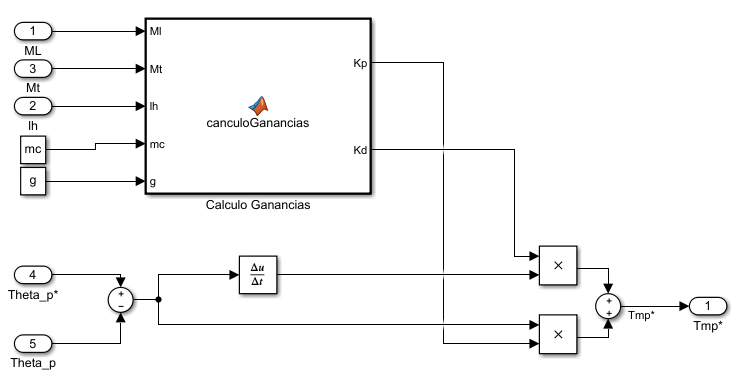
\includegraphics[width=1\textwidth]{images/imagen_15_controlador_pendulo.png}
	\caption{Diagrama de Simulink del controlador del péndulo.}
	\label{fig:controlador_pendulo}
\end{figure}

\newpage

\subsection{Nivel 1 - Control supervisor}

El controlador de nivel 1 es el encargado de supervisar los estados discretos del autómata activado por eventos y coordinar la operación suave y eficiente de los subsistemas. Este controlador cuenta con una estructura jerárquica y concurrente, lo que le permite manejar diferentes tareas de manera simultánea y coordinada.

El autómata de nivel 1 se encarga de diseñar los ciclos de operación, generar trayectorias, calcular velocidades y manejar los comandos del usuario, entre otras funciones. Una de sus tareas más importantes es enviar las consignas de velocidad a los subsistemas de carro e izaje en función del estado y posición de la carga, siguiendo una trayectoria previamente generada y actualizándola durante el movimiento.

Para lograr esto, se utilizó la herramienta StateFlow, que permitió estructurar 8 estados concurrentes principales (\textbf{Marcha, Cable Flojo, Longitud Lh, Pos Container, Freno, Control Balanceo, Frenado Seguridad}). En la figura \ref{fig:nivel_1} se puede observar el autómata y a continuación se explican detalladamente cada uno de los 8 estados.

\begin{itemize}

	\item \textbf{Nivel 1 /\ Marcha:} Es el estado principal que coordina la operación de la grúa. Acá se analiza si la grúa está \textbf{Cargado} (con contenedor) o \textbf{Descargado} (sin contenedor). Además podemos pasar al modo de \textbf{Operación} donde existen 2 tareas concurrentes: la de \textbf{Modo} que puede ser automático o manual; y \textbf{Trayectoria} que según si estamos en manual o automático planifica el control y la trayectoria.
	
	\item \textbf{Nivel 1 /\ Marcha /\ Carga:} Es el primer estado del sistema, acá se resetean todas las variables y comenzamos por verificar el estado del sistema para determinar si está \textbf{Cargado} o \textbf{Descargado}. Además una vez que estamos cargados se procede a pesar la carga, luego hacemos el seteo de las velocidades máximas para mantener la curva de potencia constante (\textbf{Velocidad}). Y tenemos una acción extra para detectar si estamos en una condición de \textbf{Sobrepeso} o no. Ver figura \ref{fig:nivel_1_carga}.
	
	\item \textbf{Nivel 1 /\ Marcha /\ Operación /\ Modo:}  Es el encargado de determinar cuando operamos en un modo u otro. Si es \textbf{Manual} el operario no podrá superar las velocidades asignadas. El modo \textbf{Automático} se activa cuando salimos de la envolvente. Ver figura \ref{fig:nivel_1_modo}.
	
	\item \textbf{Nivel 1 /\ Marcha /\ Operación /\ Trayectoria:} En este modo se coordina el seguimiento de la trayectoria. Tenemos un proceso de \textbf{Calculo Posición} que determina las etapas del movimiento desde su posición inicial, el movimiento de \textbf{Hosting}, y hasta el final. También analiza si estamos en una trayectoria simple o combinada. Ver figura \ref{fig:nivel_1_trayectoria}.
	
	\item \textbf{Nivel 1 /\ Cable Flojo:} Es un bucle que nos indica cuando el cable está flojo o sin tensión. Esto es útil para mantener un estado de operación seguro y coherente ya que si el cable permanece flojo este se puede salir. A la vez nos sirve para determinar cuando el Twist Lock se puede abrir o cerrar para tomar o dejar el contenedor. Ver figura \ref{fig:nivel_1_cable_flojo}.
	
	\item \textbf{Nivel 1 /\ Longitud Lh:} Es un ciclo encargado de corregir en tiempo real la altura medida en función de si tenemos tomado o no un contenedor. Ver figura \ref{fig:nivel_1_longitud_lh}.
	
	\item \textbf{Nivel 1 /\ Pos Container:} Es un bucle que calcula la posición del contenedor en función de la posición del carro y el ángulo theta medido. También proporciona un margen de seguridad en la envolvente. Ver figura \ref{fig:nivel_1_pos_container}.
	
	\item \textbf{Nivel 1 /\ Freno:} Es el que coordina cuando abrir o cerrar los frenos tanto de operación como de emergencia. Aunque en el \textbf{Nivel 0} hay otro control adicional de los frenos en casos de emergencia del sistema o condiciones de operación peligrosas. Ver figura \ref{fig:nivel_1_freno}.
	
	\item \textbf{Nivel 1 /\ Control Balanceo:} Es un bucle que activa o desactiva en el \textbf{Nivel 2} el control del balanceo, según el ángulo medido. Ver figura \ref{fig:nivel_1_control_balanceo}.
	
	\item \textbf{Nivel 1 /\ Frenado Seguridad:} Es un proceso en donde se hace un frenado preventivo cuando detectamos que la posición tanto del carro como del izaje están llegando a alguno de sus límites operativos. Empieza a frenar por seguridad para no chocar. Adicional a esto si se llegara a chocar por alguna razon o llegaramos a los límites responde el \textbf{Nivel 0}. Ver figura \ref{fig:nivel_1_frenado_seguridad}.
	
\end{itemize}

\begin{figure}[!h]
	\centering
	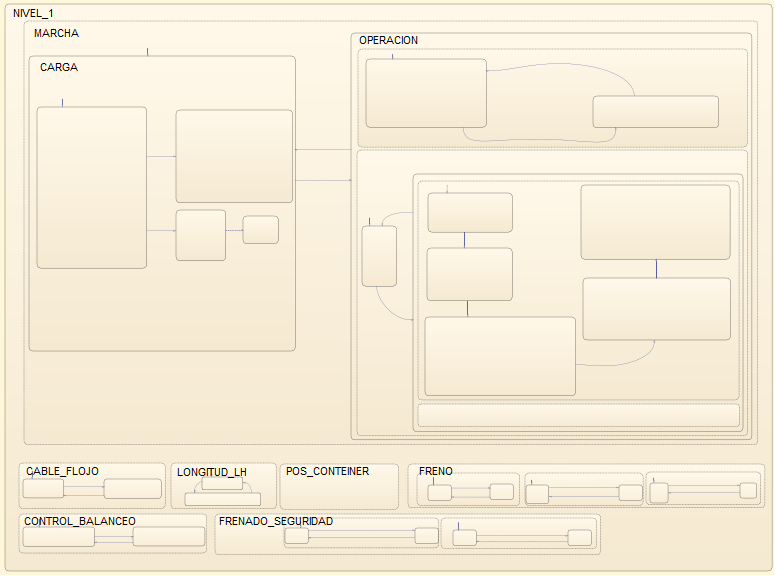
\includegraphics[width=0.9\textwidth]{images/stateflow_nivel_1/controlador_nivel1.png}
	\caption{Diagrama de StateFlow del controlador de Nivel 1.}
	\label{fig:nivel_1}
\end{figure}

\begin{figure}
	\centering
	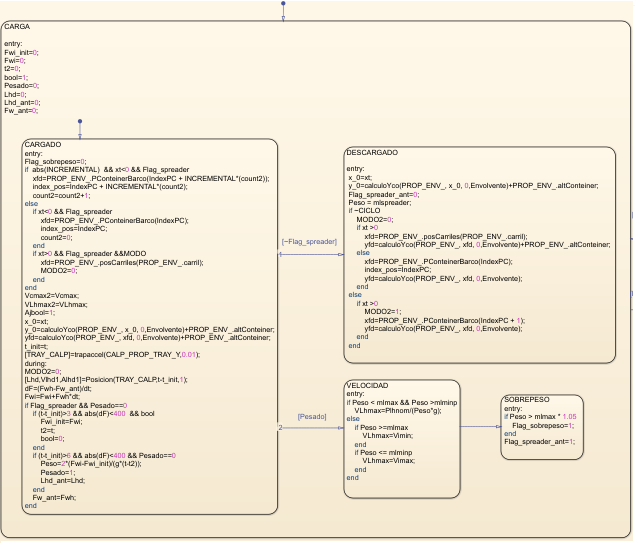
\includegraphics[width=1\textwidth]{images/stateflow_nivel_1/controlador_nivel1_carga.png}
	\caption{Diagrama de StateFlow del controlador \textbf{Nivel 1 /\ Marcha /\ Carga}.}
	\label{fig:nivel_1_carga}
\end{figure}

\begin{figure}
	\centering
	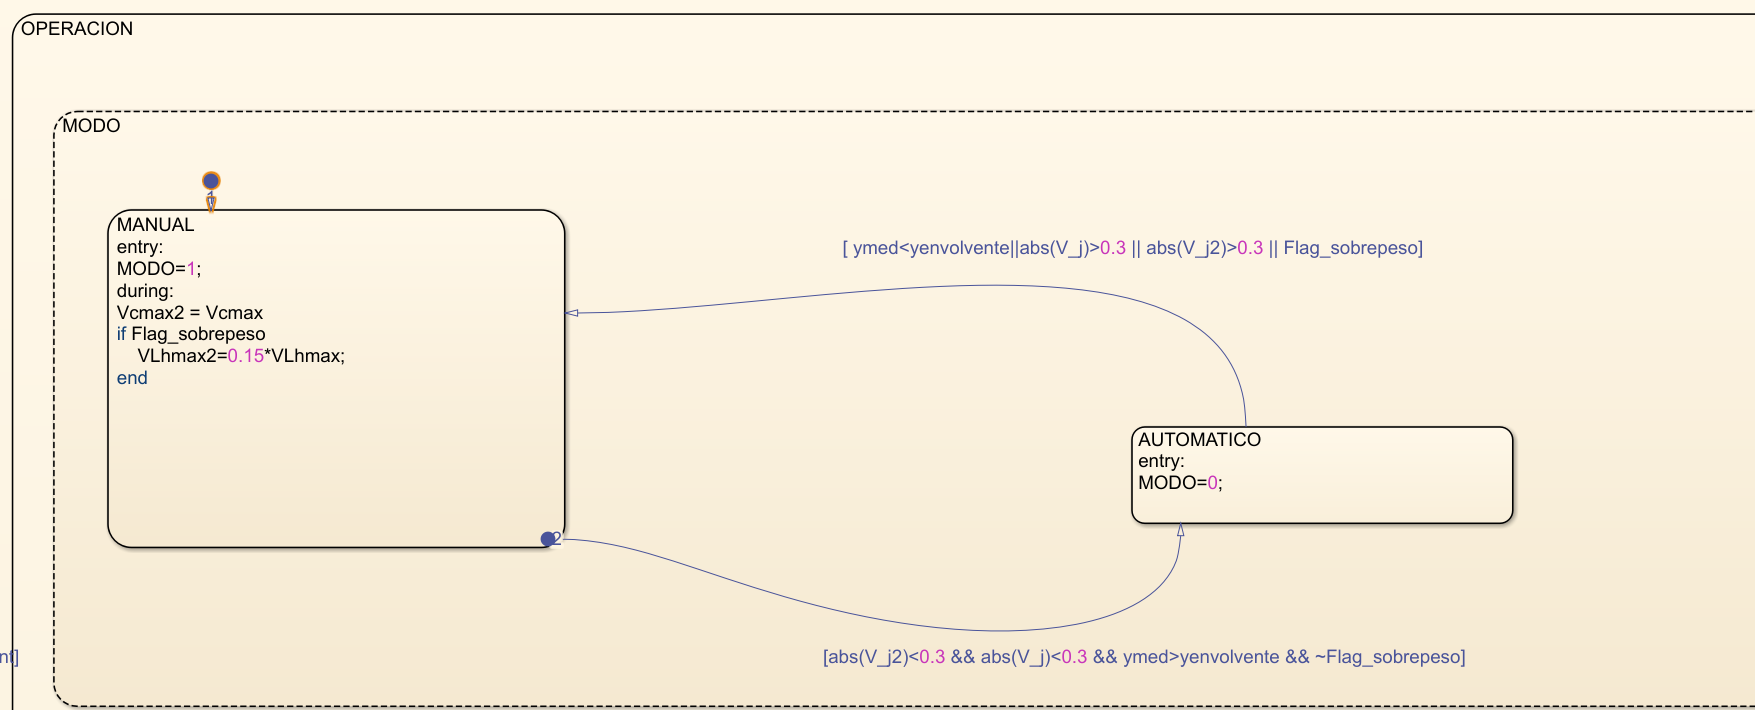
\includegraphics[width=1\textwidth]{images/stateflow_nivel_1/controlador_nivel1_operacion_modo.png}
	\caption{Diagrama de StateFlow del controlador \textbf{Nivel 1 /\ Marcha /\ Operación /\ Modo}.}
	\label{fig:nivel_1_modo}
\end{figure}

\begin{figure}
	\centering
	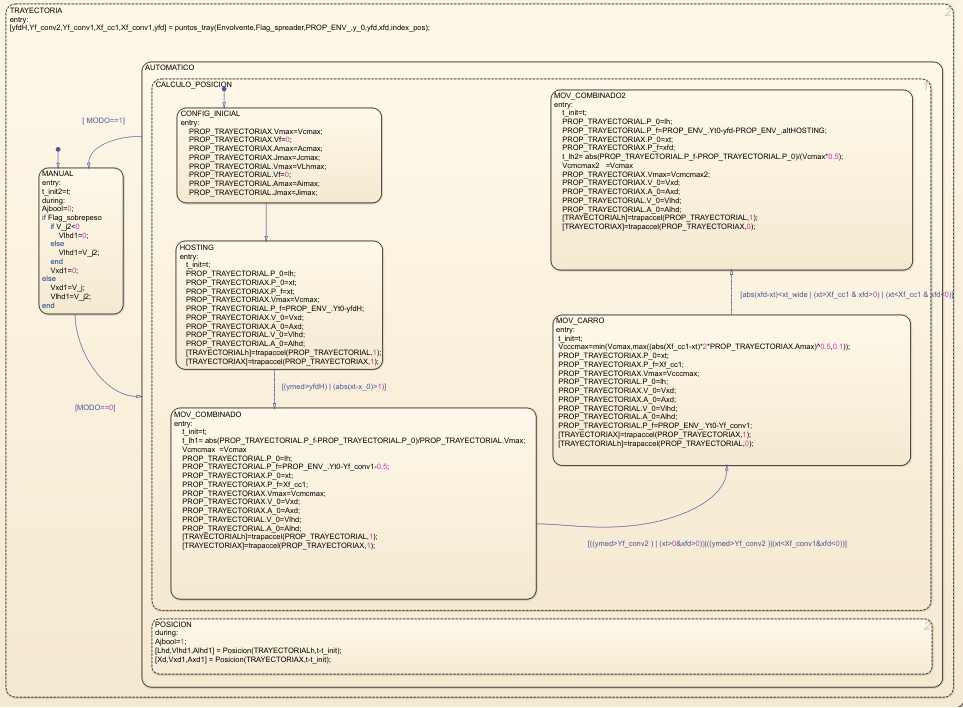
\includegraphics[width=1\textwidth]{images/stateflow_nivel_1/controlador_nivel1_operacion_trayectoria.png}
	\caption{Diagrama de StateFlow del controlador \textbf{Nivel 1 /\ Marcha /\ Operacion /\ Trayectoria}.}
	\label{fig:nivel_1_trayectoria}
\end{figure}

\begin{figure}
	\centering
	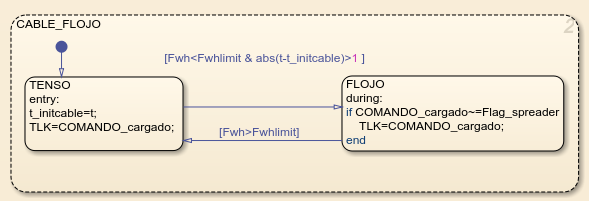
\includegraphics[width=0.8\textwidth]{images/stateflow_nivel_1/controlador_nivel1_cable_flojo.png}
	\caption{Diagrama de StateFlow del controlador \textbf{Nivel 1 /\ Cable Flojo}.}
	\label{fig:nivel_1_cable_flojo}
\end{figure}

\begin{figure}
	\centering
	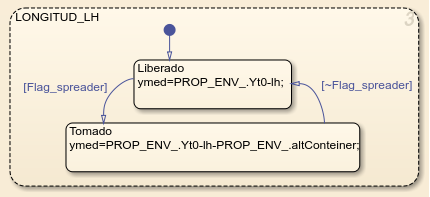
\includegraphics[width=0.55\textwidth]{images/stateflow_nivel_1/controlador_nivel1_longitud_lh.png}
	\caption{Diagrama de StateFlow del controlador \textbf{Nivel 1 /\ Longitud Lh}.}
	\label{fig:nivel_1_longitud_lh}
\end{figure}

\begin{figure}
	\centering
	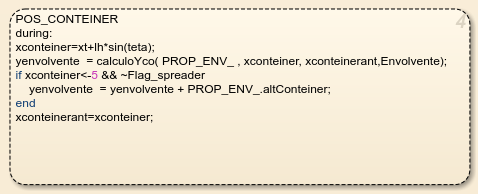
\includegraphics[width=0.7\textwidth]{images/stateflow_nivel_1/controlador_nivel1_pos_conteiner.png}
	\caption{Diagrama de StateFlow del controlador \textbf{Nivel 1 /\ Pos Container}.}
	\label{fig:nivel_1_pos_container}
\end{figure}

\begin{figure}
	\centering
	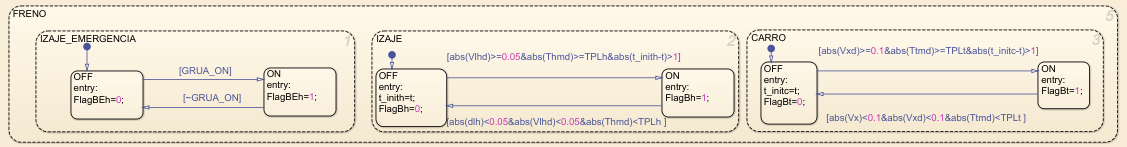
\includegraphics[width=1\textwidth]{images/stateflow_nivel_1/controlador_nivel1_freno.png}
	\caption{Diagrama de StateFlow del controlador \textbf{Nivel 1 /\ Freno}.}
	\label{fig:nivel_1_freno}
\end{figure}

\begin{figure}
	\centering
	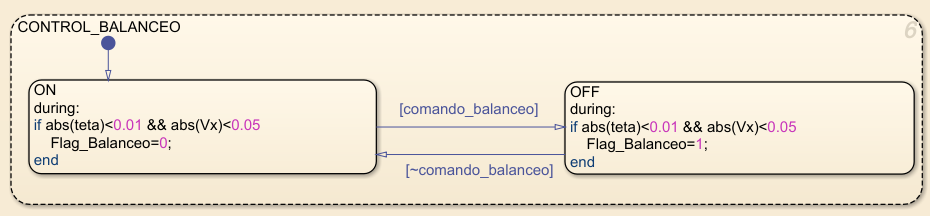
\includegraphics[width=1\textwidth]{images/stateflow_nivel_1/controlador_nivel1_control_balanceo.png}
	\caption{Diagrama de StateFlow del controlador \textbf{Nivel 1 /\ Control Balanceo}.}
	\label{fig:nivel_1_control_balanceo}
\end{figure}

\begin{figure}
	\centering
	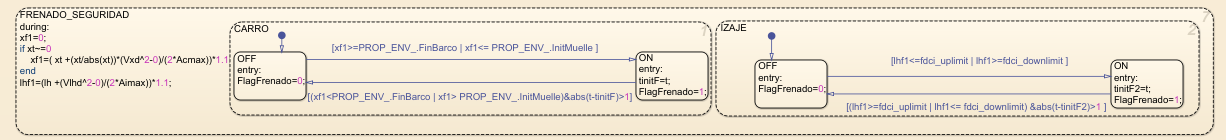
\includegraphics[width=1\textwidth]{images/stateflow_nivel_1/controlador_nivel1_freno_seguridad.png}
	\caption{Diagrama de StateFlow del controlador \textbf{Nivel 1 /\ Frenado Seguridad}.}
	\label{fig:nivel_1_frenado_seguridad}
\end{figure}

\newpage

En conclusión, el controlador de \textbf{Nivel 1} es una parte fundamental del sistema de control ya que es el coordinador de toda la operación de la maquina, es el encargado de supervisar y coordinar la operación suave y eficiente de los subsistemas en función del estado y posición de la carga. Su estructura jerárquica y concurrente, le permite manejar diferentes tareas de manera simultánea y coordinada.

\subsection{Nivel 0 - Control de seguridad}

El autómata de \textbf{Nivel 0} está diseñado para garantizar la detención inmediata del sistema en caso de emergencia y poder llevar al mismo a un estado seguro. Este autómata se divide en dos estados concurrentes, los cuales se encargan de verificar las condiciones de seguridad y detener el sistema en caso de ser necesario. En la figura \ref{fig:nivel_0} se puede observar el autómata diseñado.

Es importante destacar que el controlador de \textbf{Nivel 0} debe estar diseñado de manera adecuada y cumplir con los estándares de seguridad establecidos, para garantizar una operación segura y eficiente del sistema.

Los dos estados concurrentes principales son:
\begin{itemize}
	\item \textbf{Emergencia:} Este ciclo es el que busca problemas o posibles estados de falla en el sistema y si los encuentra lanza alertas en base a las señales que recibe de distintos sensores y/o botones que tiene el operario.
	\item \textbf{Watchdog:} Es el ciclo que se encarga de detectar errores en la ejecución del controlador y actualizar las variables para indicar los estados necesarios.
\end{itemize}

\begin{figure}[!h]
	\centering
	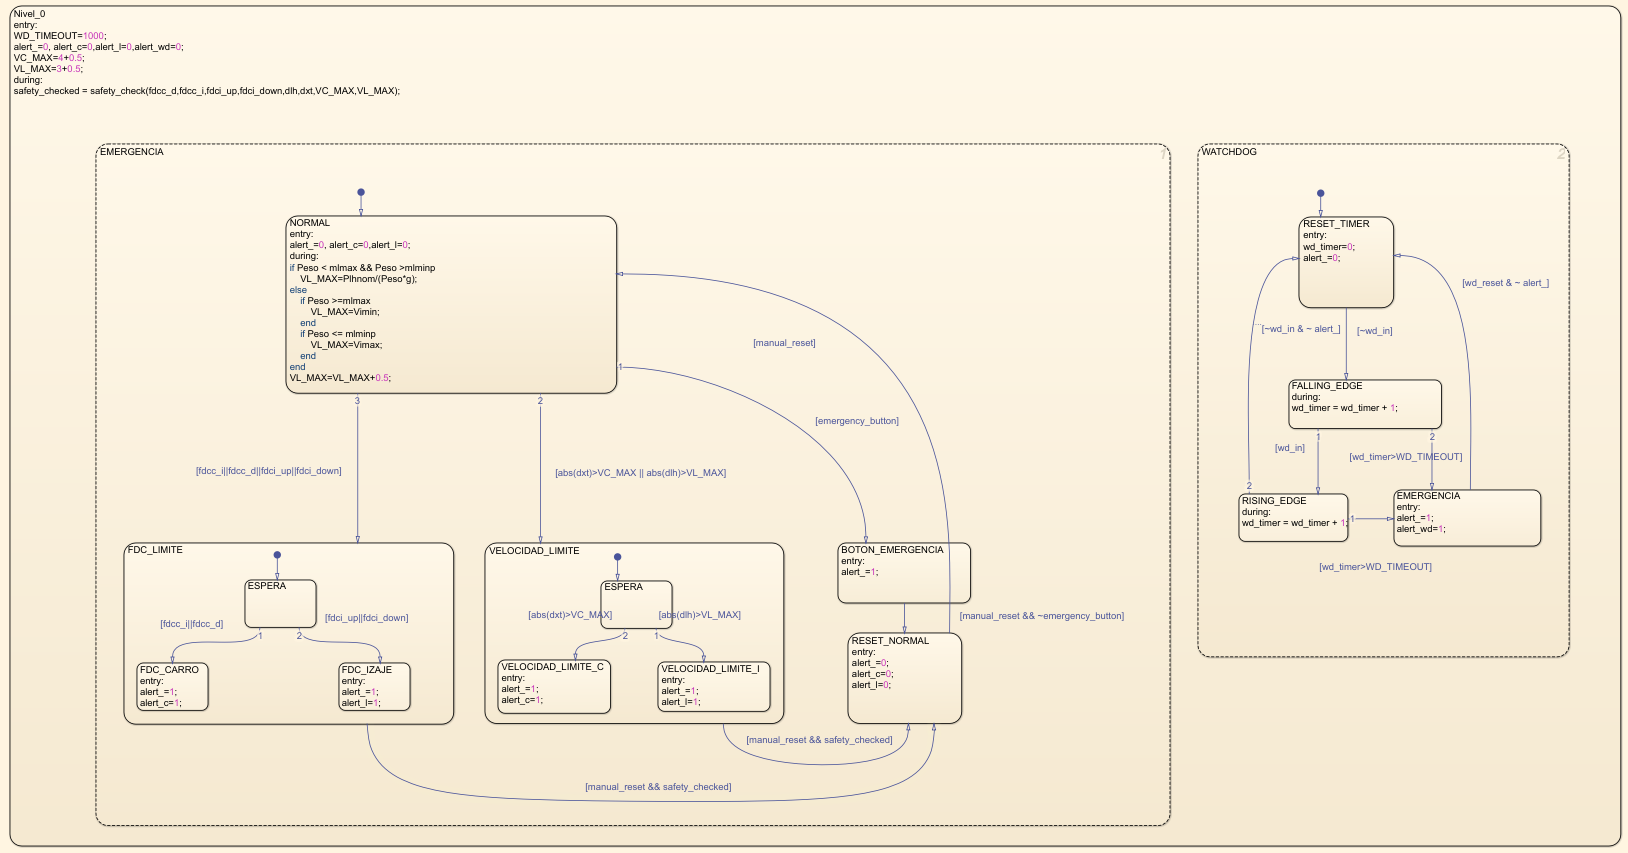
\includegraphics[width=1\textwidth]{images/imagen_26_nivel_0.png}
	\caption{Diagrama de StateFlow del controlador \textbf{Nivel 0}.}
	\label{fig:nivel_0}
\end{figure}

El automatismo de \textbf{Nivel 0}, tiene como objetivo monitorear la posición y velocidad de los subsistemas de carro y de izaje, con el fin de evitar cualquier irregularidad que pueda ocurrir durante su operación. Se han considerado tres casos posibles en los que se activaría una emergencia. Los mismos son los siguientes:

\begin{itemize}
	\item En el primer caso, si la \textbf{velocidad} del sistema de izaje o del carro supera sus valores \textbf{máximos permitidos}, se activan unas señales de alerta que automáticamente envían una consigna a los frenos de seguridad para que se cierren (frenen al sistema). Y se desactiva el controlador de \textbf{Nivel 2}.

	\item En el segundo caso, si el carro o el sistema de izaje alcanzan sus \textbf{límites físicos}, los fines de carrera se activan y, junto con ellos, el sistema de freno de emergencia. En este caso se procede igual que en el caso anterior deteniendo el sistema completamente para evitar cualquier daño o riesgo de seguridad.
	
	\item En el tercer caso, si el \textbf{operario} al mando necesita detener el sistema por cualquier razón que considere, puede activar el \textbf{pulsador de emergencia}, lo que también activará el sistema de frenado de emergencia y detendrá el sistema por completo.
\end{itemize}

\begin{figure}[!h]
	\centering
	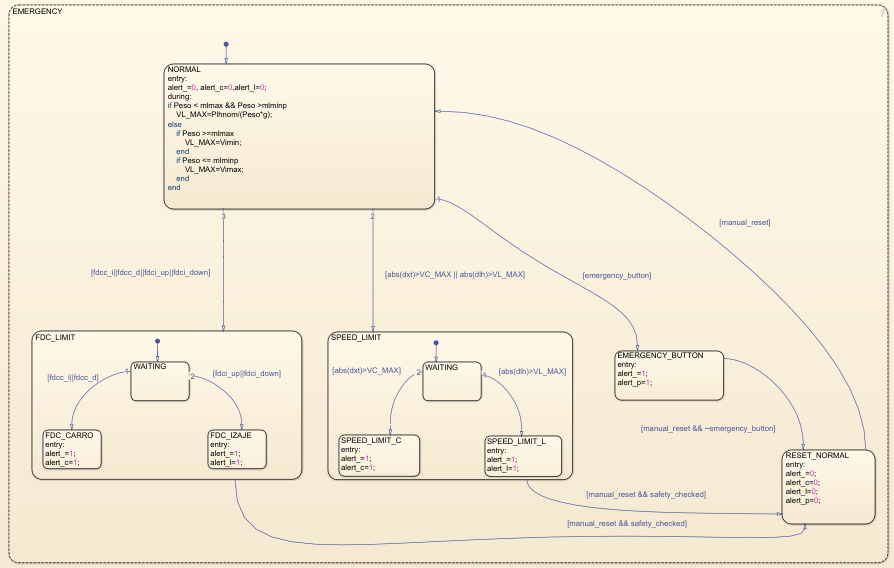
\includegraphics[width=1\textwidth]{images/imagen_27_emergencia.png}
	\caption{Diagrama de StateFlow de la rutina de \textbf{Emergencia} del \textbf{Nivel 0}.}
	\label{fig:nivel_0_emergencia}
\end{figure}

En relación a los casos anteriormente mencionados, en todos se generan dos tipos de alertas al detectar una irregularidad en el sistema: una alerta general y una alerta específica que varía en función de la causa de la irregularidad. Estas variables se pueden observar en el automatismo con los siguientes nombres:

\begin{itemize}
	\item \texttt{alert\_}: Es la señal general de alerta. La misma se activa siempre que haya un estado de emergencia.
	\item \texttt{alert\_i}: Se activa si la causa de la emergencia es en el carro.
	\item \texttt{alert\_c}: Se activa si la causa de la emergencia es en el izaje.
	\item \texttt{alert\_p}: Se activa si la emergencia fue accionada por el pulsador del operario.
	\item \texttt{alert\_wd}: Se activa cuando la alerta es disparada por el Watchdog.
\end{itemize}

Adicionalmente, el mecanismo de vigilancia (o Watchdog) es responsable de reiniciar un contador cada vez que detecta cambios en el pulso proveniente de un reloj externo. En caso de que la ejecución del programa experimente alguna dificultad, el contador no se reiniciará, y si llega a alcanzar un valor preestablecido, se detendrá el sistema. Disparando la alarma correspondiente. Esto se puede ver en el diagrama de la figura \ref{fig:nivel_0_watchdog}.

\begin{figure}[!h]
	\centering
	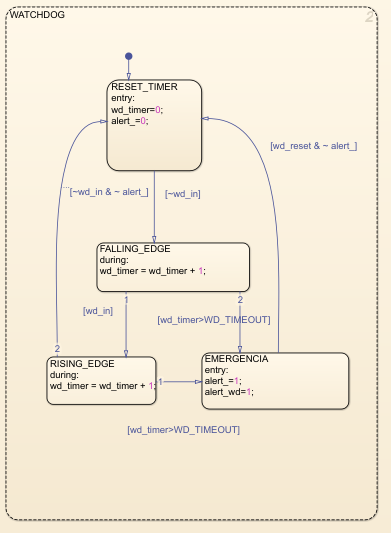
\includegraphics[width=0.5\textwidth]{images/imagen_28_watchdog.png}
	\caption{Diagrama de StateFlow de la rutina de \textbf{Watchdog} del \textbf{Nivel 0}.}
	\label{fig:nivel_0_watchdog}
\end{figure}

\newpage

Además como mencionamos anteriormente una de las posibilidades para disparar una alerta es que el operario active la alarma con una señal de emergencia. Esto se hace utilizando los siguientes pulsadores:
\begin{itemize}
	\item El operario active la alarma con una señal de emergencia. Usando el \textbf{pulsador de emergencia}.
	\item Luego de esto deberá presionar un \textbf{pulsador de reset} si quiere que el sistema arranque desde cero luego de haberse disparado la alarma. Como se ve en la figura \ref{fig:nivel_0_emergencia}
\end{itemize}

\section{Simulación}
En este apartado se presentarán los resultados de las simulaciones realizadas en el proyecto, en las cuales se puso a prueba el trabajo conjunto de los tres niveles de control para lograr las trayectorias deseadas. A partir de las simulaciones, se identificó que las trayectorias pueden ser optimizadas para que el contenedor se acerque más a las columnas de contenedores, con el objetivo de reducir tanto el tiempo como el consumo de energía en el proceso. En las siguientes secciones se detallarán los resultados obtenidos y las conclusiones que se pueden extraer de ellos.

\subsection{Ciclo simple a máxima carga}

En la figura \ref{fig:ciclo_simple_maxima_carga_trayectoria} se presenta el resultado obtenido tras la realización de una trayectoria de ciclo simple, con una carga máxima de $65.000\ Kg$, considerando el contenedor más el spreader. En esta simulación, el movimiento se inicia desde el lado del muelle, trasladando el contenedor hacia la última columna del barco para luego volver al punto de partida. Cabe destacar que el sistema logró llevar a cabo esta tarea de forma satisfactoria, cumpliendo con los objetivos planteados en cuanto a la trayectoria y la carga soportada. Los resultados obtenidos en esta simulación permiten validar la capacidad del sistema para enfrentar tareas de carga y descarga en situaciones reales de trabajo en puerto.

\begin{figure}[!h]
	\centering
	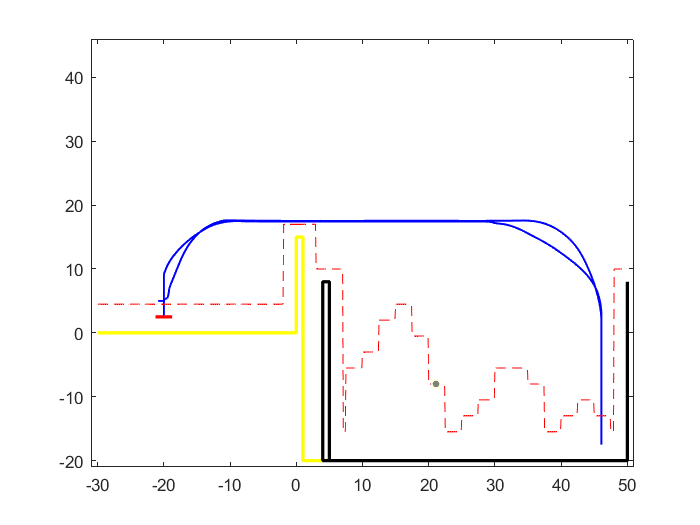
\includegraphics[width=1\textwidth]{images/ciclo_simple_maxima_carga/trayectoria_completa_xtd.png}
	\caption{Trayectoria de ciclo simple con carga máxima.}
	\label{fig:ciclo_simple_maxima_carga_trayectoria}
\end{figure}

En relación a la simulación de la trayectoria con carga máxima, se determinó que la velocidad de izaje máxima posible es de $1.5\ m/s$, tal como se observa en la figura \ref{fig:ciclo_simple_maxima_carga_velocidad_izaje}. Por otro lado, la velocidad máxima de traslado horizontal permitida en esta situación es de $4\ m/s$, como se muestra en la figura \ref{fig:ciclo_simple_maxima_carga_velocidad_carro}. Esta restricción en las velocidades de movimiento tiene como finalidad mantener la potencia de funcionamiento constante durante el movimiento vertical, garantizando así la estabilidad y seguridad del sistema en todo momento. De esta manera, se asegura que el sistema pueda trabajar de manera eficiente y segura en situaciones de carga máxima.

\begin{figure}%[!h]
	\centering
	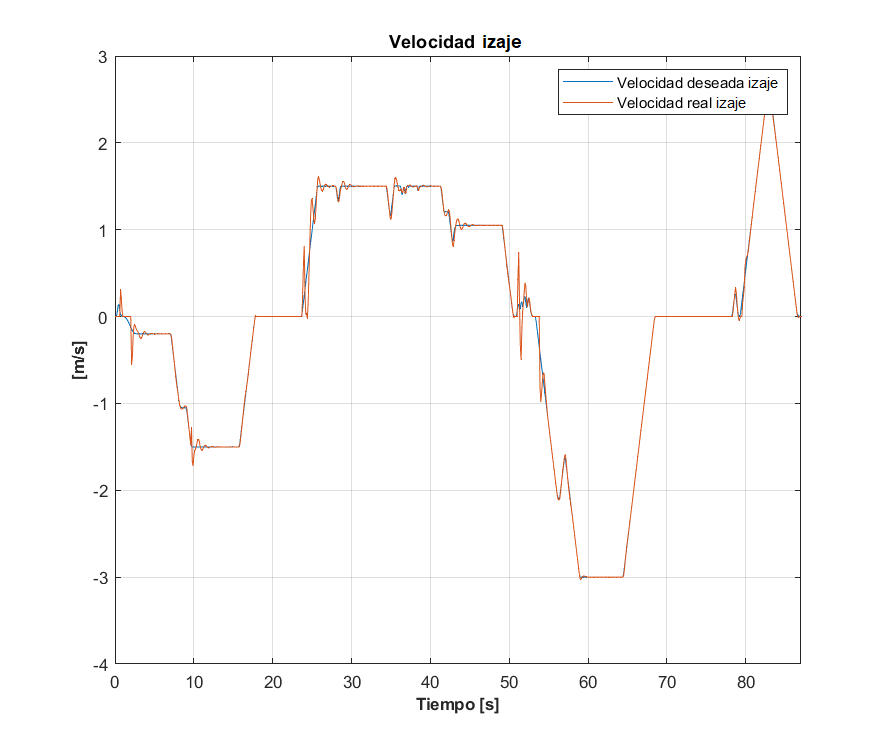
\includegraphics[width=0.9\textwidth]{images/ciclo_simple_maxima_carga/velocidad_izaje_fix.png}
	\caption{Velocidad de izaje. Ciclo simple con carga máxima.}
	\label{fig:ciclo_simple_maxima_carga_velocidad_izaje}
\end{figure}

\begin{figure}%[!h]
	\centering
	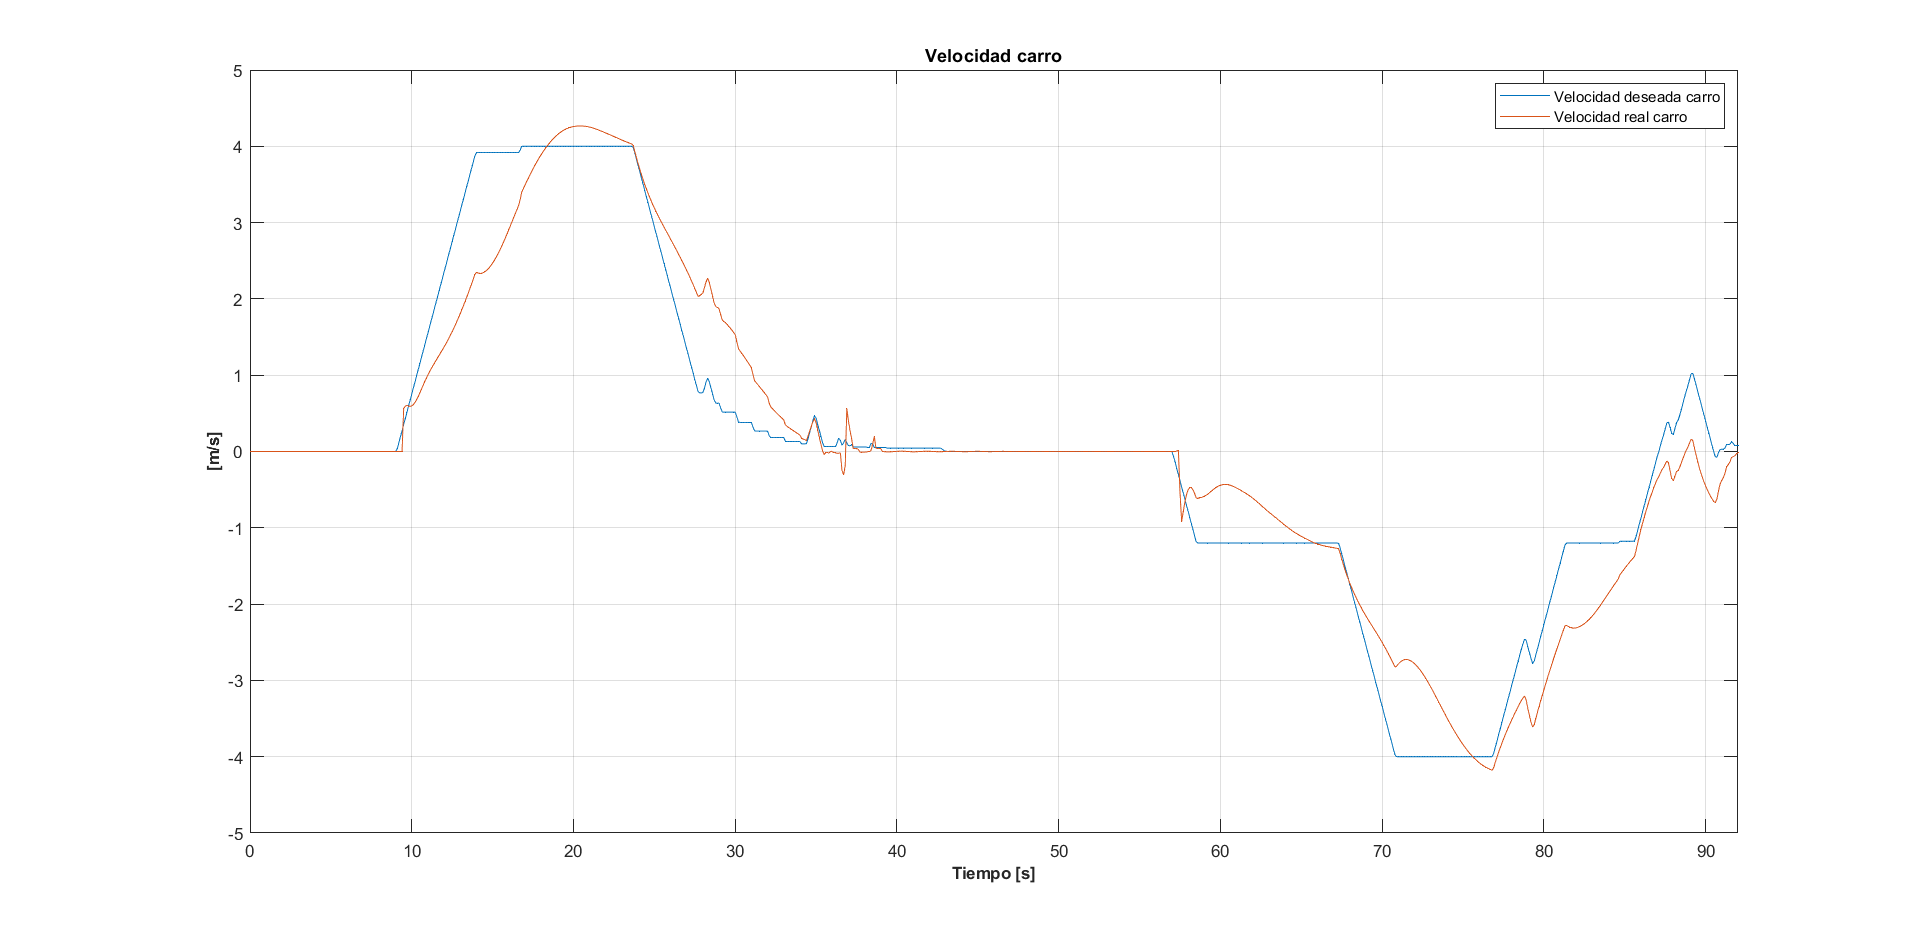
\includegraphics[width=1\textwidth]{images/ciclo_simple_maxima_carga/velocidad_carro.png}
	\caption{Velocidad del carro. Ciclo simple con carga máxima.}
	\label{fig:ciclo_simple_maxima_carga_velocidad_carro}
\end{figure}

En el primer tramo de la figura \ref{fig:ciclo_simple_maxima_carga_velocidad_izaje}, se puede apreciar una velocidad reducida de $0.15\ m/s$ para permitir una elevación suave del contenedor desde el suelo, hasta que la masa sea estimada. A partir de los 10 segundos, la velocidad aumenta a $1.5\ m/s$, lo cual depende del valor de la carga que se está trasladando. Durante el tramo de vuelta al barco (desde los 60 segundos en adelante), cuando el ``spreader'' regresa sin carga, la velocidad se duplica para mantener la potencia constante nuevamente.

En la figura \ref{fig:ciclo_simple_maxima_carga_velocidad_carro}, se puede apreciar que el carro sigue la consigna de velocidad en los tramos donde no hay cambios de consigna. Sin embargo, en los puntos de transición, hay un retraso en el seguimiento de la consigna por parte del sistema debido al efecto del control de balanceo.

Por otro lado, en la figura \ref{fig:ciclo_simple_maxima_carga_angulo_balanceo}, se muestra el ángulo de balanceo de la carga. El sistema de control empleado presenta un rendimiento aceptable, buscando reducir el ángulo lo más rápido posible durante alguna desviación del 0. Es importante destacar que se cumplen los requerimientos planteados, ya que el ángulo no supera los $20°$ durante los cambios de posición y se restablece rápidamente a $0°$ después de algún cambio de consigna.

En la figura \ref{fig:ciclo_simple_maxima_carga_fza_cable} se muestra la variación de la fuerza de tensión del cable a lo largo del trayecto. Es importante mencionar que se observa un retraso en la estabilización de la fuerza, lo que requiere la utilización de la integral de su valor para estimar la masa tempranamente. De esta forma, se puede obtener una estimación precisa y rápida de la masa en movimiento. Cabe destacar que este comportamiento ha sido contemplado en el diseño del sistema de control para garantizar la precisión y eficacia del mismo en todo momento.

\begin{figure}%[!h]
	\centering
	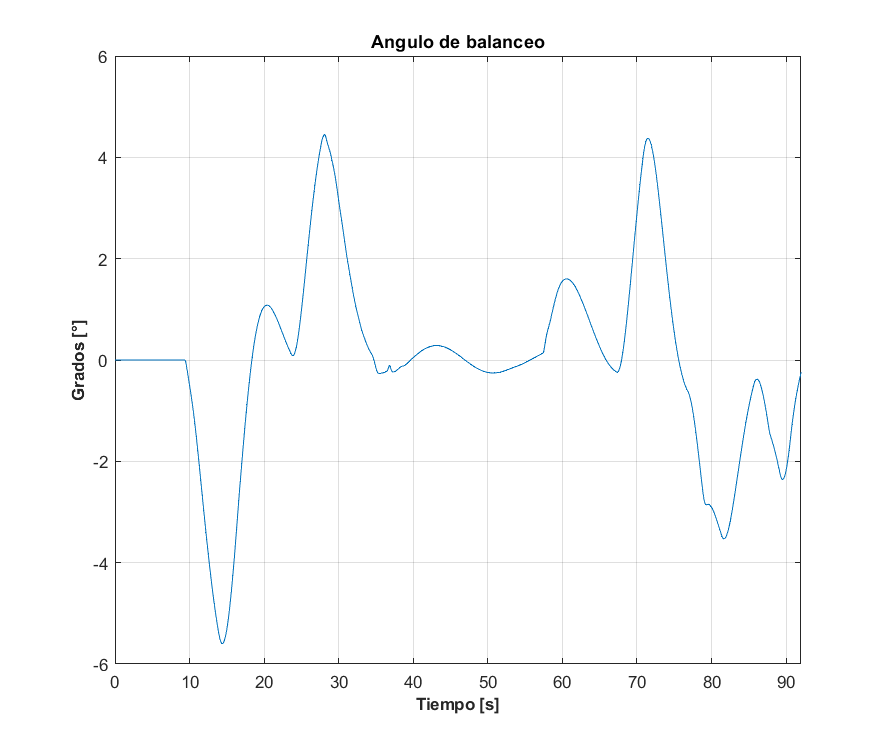
\includegraphics[width=0.7\textwidth]{images/ciclo_simple_maxima_carga/angulo_de_balanceo.png}
	\caption{Ángulo de balanceo de carga. Ciclo simple con carga máxima.}
	\label{fig:ciclo_simple_maxima_carga_angulo_balanceo}
\end{figure}

\begin{figure}%[!h]
	\centering
	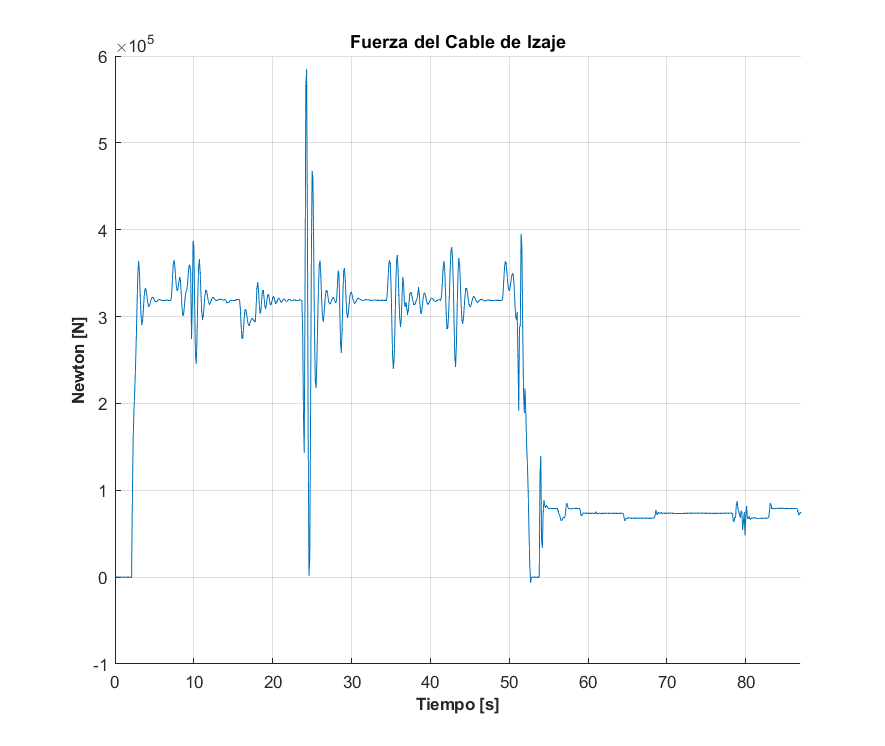
\includegraphics[width=0.8\textwidth]{images/ciclo_simple_maxima_carga/FuerzadeIzaje.png}
	\caption{Fuerza de tensión del cable. Ciclo simple con carga máxima.}
	\label{fig:ciclo_simple_maxima_carga_fza_cable}
\end{figure}

\subsection{Ciclo doble a media carga}

En la figura \ref{fig:ciclo_doble_media_carga_trayectoria} se puede observar que la trayectoria de ciclo doble se realiza de manera satisfactoria. El primer tramo, desde el muelle hasta que deja el primer contenedor, se realiza de manera automática, luego en el segundo tramo, el ``spreader'' se mueve de forma manual pero sin carga para buscar el próximo contenedor y ahí se activan los ``twistlocks'' para sujetar este contenedor y llevarlo al muelle de forma automática.

Es importante destacar que la transición entre los tramos se realiza de manera suave y sin problemas, lo cual indica que el sistema de control utilizado es adecuado para este tipo de operaciones. Además, se puede apreciar que la velocidad de izaje máxima en el tramo de ida es mayor que en la simulación anterior (figura \ref{fig:ciclo_simple_maxima_carga_velocidad_izaje}), lo que demuestra la capacidad del sistema para ajustar la velocidad en función de la carga transportada para mantener la curda de potencia constante.

\begin{figure}[!h]
	\centering
	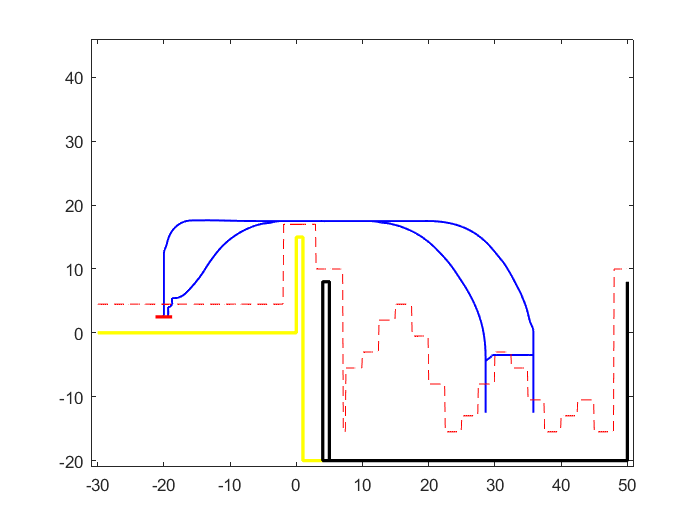
\includegraphics[width=1\textwidth]{images/ciclo_doble_carga_media/trayectoria_completa_xtd - copia.png}
	\caption{Trayectoria de ciclo doble con carga media.}
	\label{fig:ciclo_doble_media_carga_trayectoria}
\end{figure}

Así como mencionamos antes, a continuación se muestran las velocidades del carro e izaje en las figuras \ref{fig:ciclo_doble_media_carga_velocidad_izaje} y \ref{fig:ciclo_doble_media_carga_velocidad_carro}.

\begin{figure}%[!h]
	\centering
	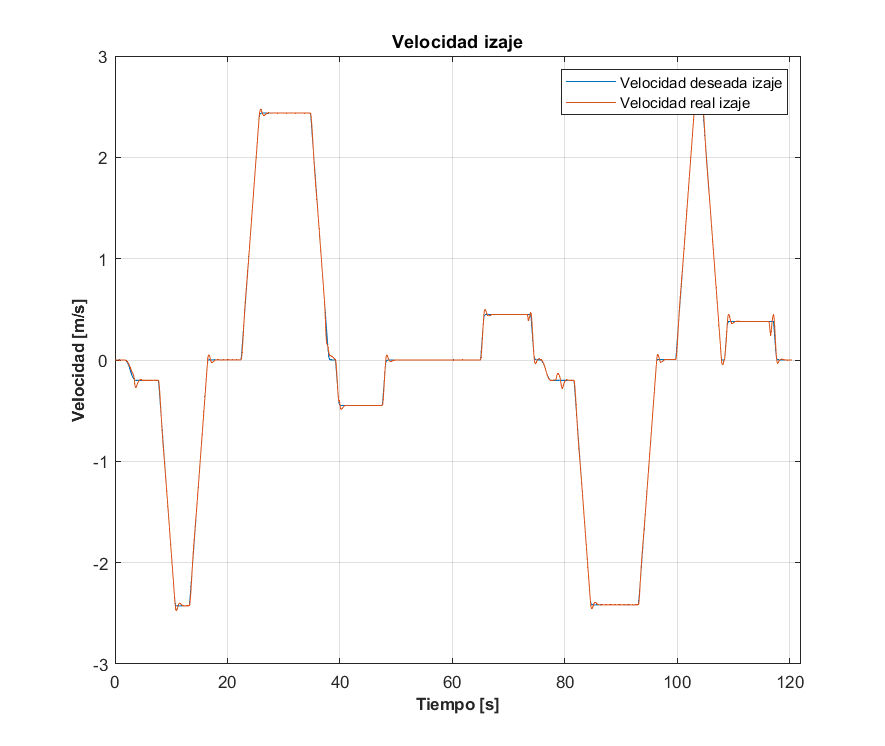
\includegraphics[width=1\textwidth]{images/ciclo_doble_carga_media/velocidad_izaje - copia.png}
	\caption{Velocidad de izaje. Ciclo doble con carga media.}
	\label{fig:ciclo_doble_media_carga_velocidad_izaje}
\end{figure}

\begin{figure}%[!h]
	\centering
	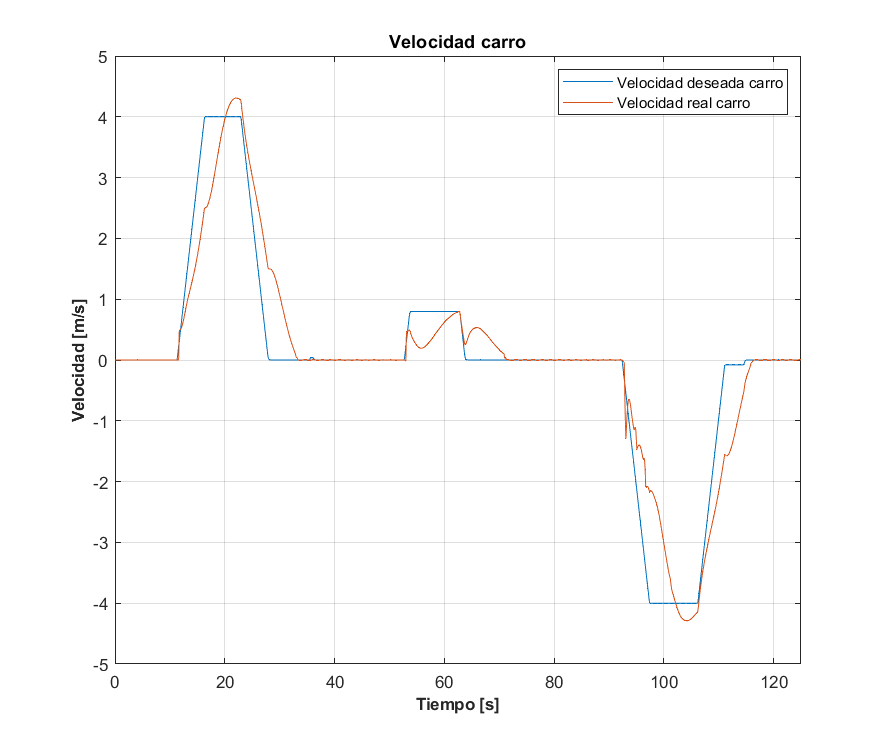
\includegraphics[width=1\textwidth]{images/ciclo_doble_carga_media/velocidad_carro.png}
	\caption{Velocidad del carro. Ciclo doble con carga media.}
	\label{fig:ciclo_doble_media_carga_velocidad_carro}
\end{figure}

\newpage

\subsection{Sistema de emergencia}

En cuanto a la seguridad y protección del sistema, se llevaron a cabo pruebas de emergencia para evaluar su comportamiento en caso de situaciones críticas. De la figura \ref{fig:pulsador_emergencia_velocidad_izaje} a la \ref{fig:pulsador_emergencia_fuerza_cable_izaje} se muestra el resultado del sistema ante el accionamiento del \textbf{pulsador de emergencia}. Es posible observar cómo el sistema se detiene inmediatamente después de que se dispara la alerta (antes del segundo 5 apróx.), las consignas de velocidad pasan a 0 inmediatamente y se activan los frenos mecánicos para lograr un frenado óptimo y seguro.

\begin{figure}[!h]
	\centering
	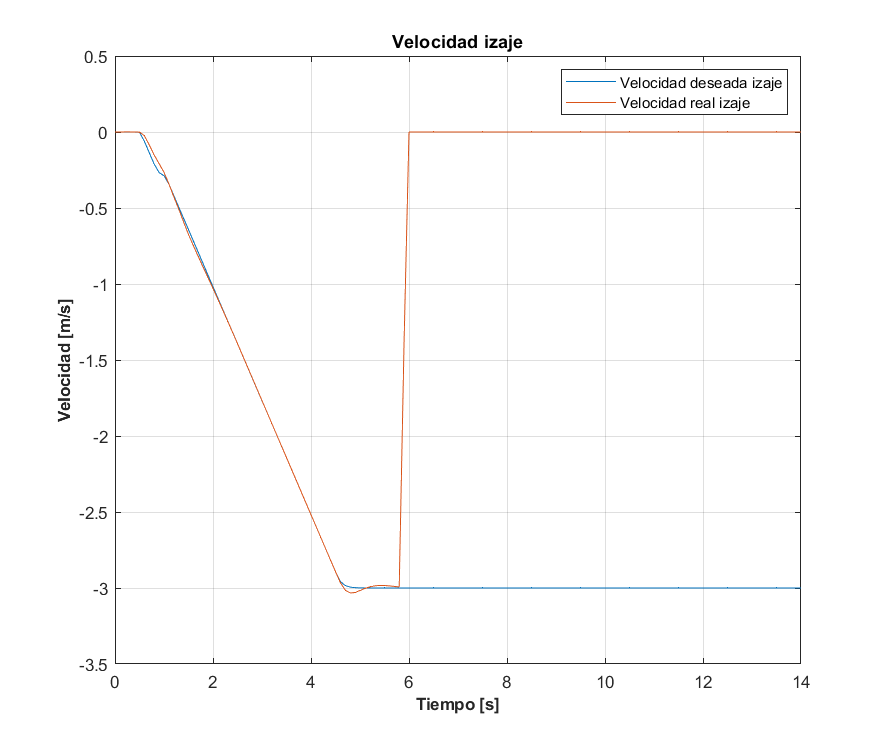
\includegraphics[width=0.6\textwidth]{images/Freno_emergencia/velocidad_izaje.png}
	\caption{Velocidad del izaje. Alerta accionada por el pulsador de emergencia.}
	\label{fig:pulsador_emergencia_velocidad_izaje}
\end{figure}

\begin{figure}[!h]
	\centering
	\includegraphics[width=0.6\textwidth]{images/Freno_emergencia/velocidad_carro.png}
	\caption{Velocidad del carro. Alerta accionada por el pulsador de emergencia.}
	\label{fig:pulsador_emergencia_velocidad_carro}
\end{figure}

\begin{figure}[!h]
	\centering
	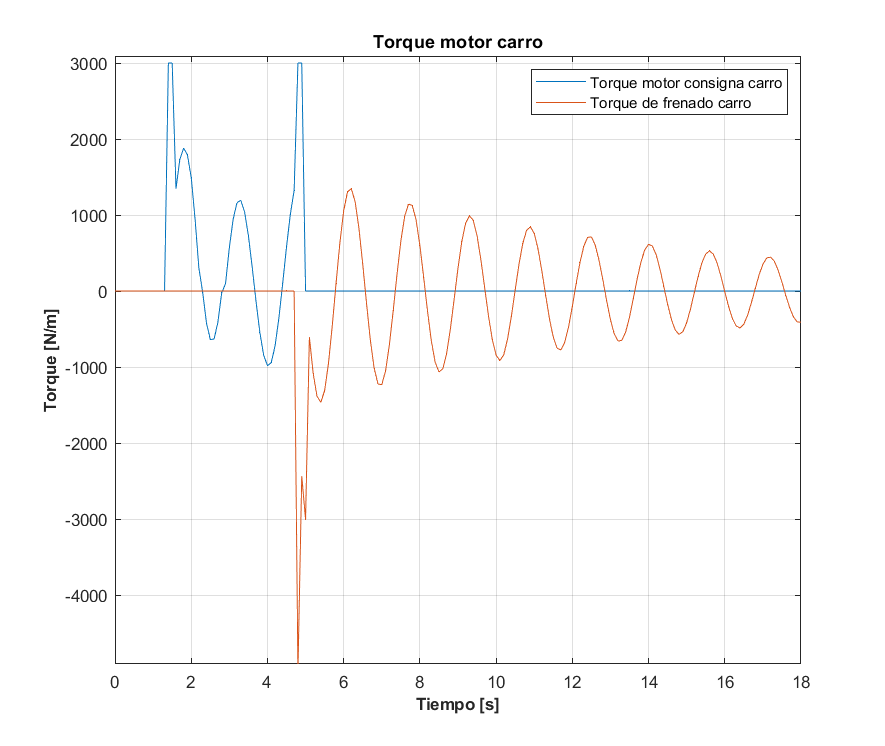
\includegraphics[width=0.6\textwidth]{images/Freno_emergencia/torque_motor_carro.png}
	\caption{Torque de frenado del carro. Alerta accionada por el pulsador de emergencia.}
	\label{fig:pulsador_emergencia_torque_motor_carro}
\end{figure}

\begin{figure}[!h]
	\centering
	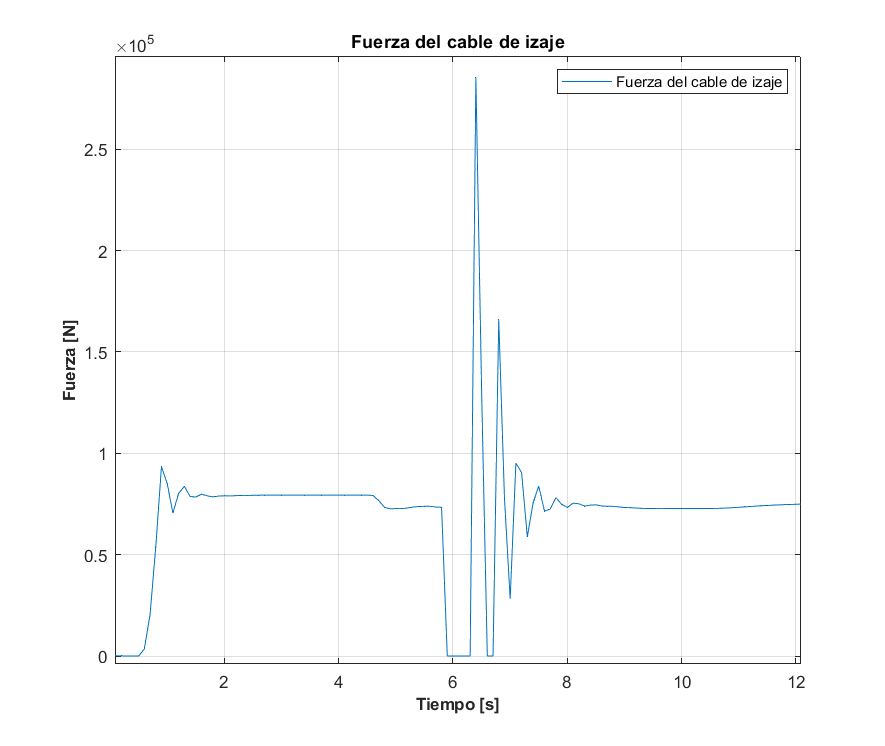
\includegraphics[width=0.6\textwidth]{images/Freno_emergencia/fuerza_cable_izaje.png}
	\caption{Fuerza del cable del izaje. Alerta accionada por el pulsador de emergencia.}
	\label{fig:pulsador_emergencia_fuerza_cable_izaje}
\end{figure}

\newpage

En el segundo caso presentado figuras \ref{fig:final_carrera_velocidad_izaje} a \ref{fig:final_carrera_fuerza_cable_izaje} se muestra la respuesta del control de nivel 0 ante la \textbf{activación} de uno de los \textbf{fines de carrera} para el movimiento horizontal. En este caso, una vez activado el fin de carrera a los 5 segundos de la simulación, el sistema muestra una respuesta casi instantanea deteniendo el movimiento en apenas fracciones de segundos. Esta detención se realiza de manera segura y sin generar situaciones de riesgo para la carga o para los operarios. Este comportamiento demuestra que el control de nivel 0 funciona adecuadamente ante situaciones de emergencia y que es capaz de detener el sistema de forma controlada y segura.

\begin{figure}[!h]
	\centering
	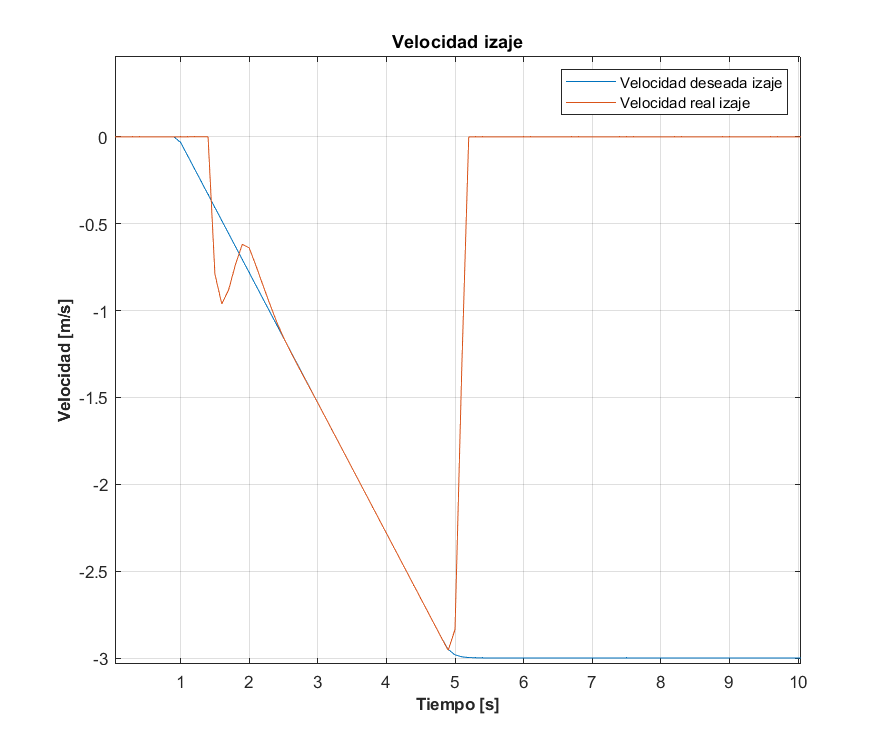
\includegraphics[width=0.75\textwidth]{images/Freno_fin_de_carrera/velocidad_izaje.png}
	\caption{Velocidad del izaje. Alerta accionada por el final de carrera.}
	\label{fig:final_carrera_velocidad_izaje}
\end{figure}

\begin{figure}[!h]
	\centering
	\includegraphics[width=0.75\textwidth]{images/Freno_fin_de_carrera/velocidad_carro.png}
	\caption{Velocidad del carro. Alerta accionada por el final de carrera.}
	\label{fig:final_carrera_velocidad_carro}
\end{figure}

\begin{figure}[!h]
	\centering
	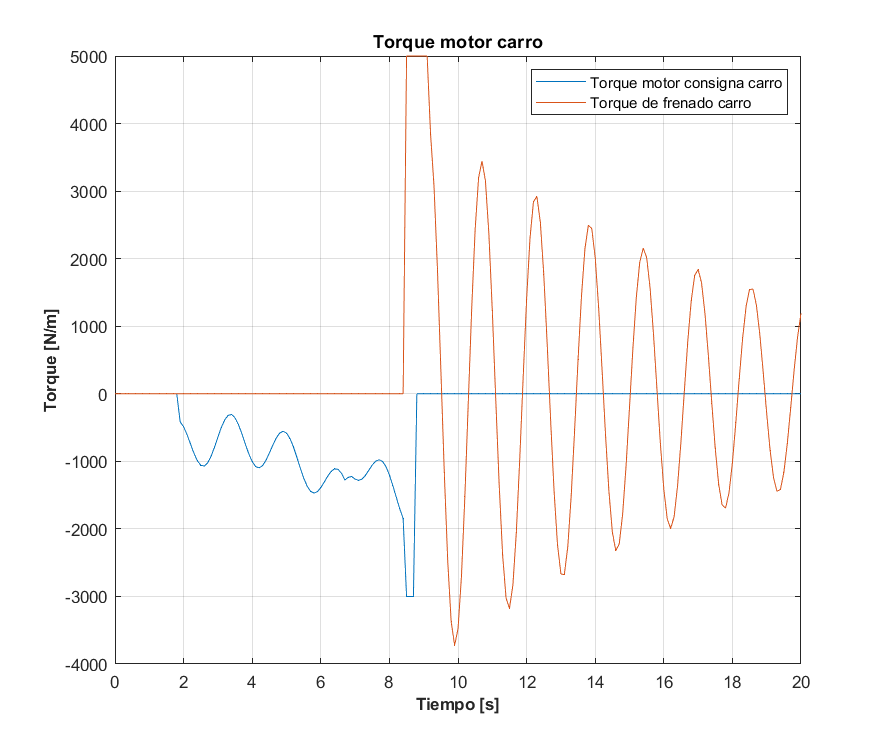
\includegraphics[width=0.6\textwidth]{images/Freno_fin_de_carrera/torque_carro.png}
	\caption{Torque de frenado del carro. Alerta accionada por el final de carrera.}
	\label{fig:final_carrera_torque_motor_carro}
\end{figure}

\begin{figure}[!h]
	\centering
	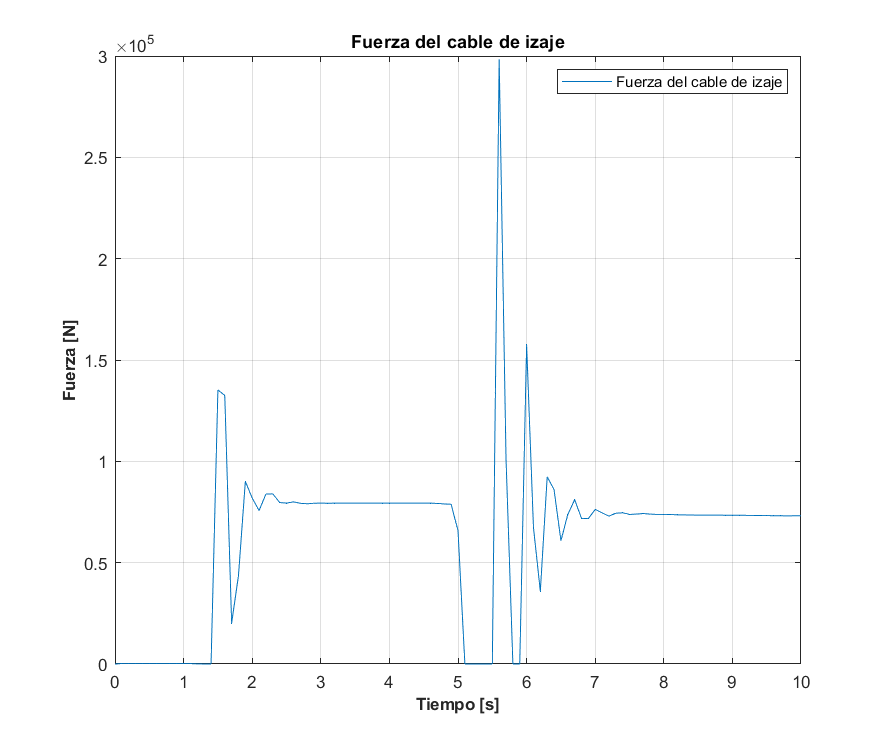
\includegraphics[width=0.6\textwidth]{images/Freno_fin_de_carrera/fuerza_izaje.png}
	\caption{Fuerza del cable del izaje. Alerta accionada por el final de carrera.}
	\label{fig:final_carrera_fuerza_cable_izaje}
\end{figure}

\newpage

En el tercer caso, el sistema también cuenta con medidas de protección ante \textbf{velocidades} de izaje o traslación que \textbf{superen las máximas permitidas}. Esto es para prevenir situaciones como la de desconexión de alguna etapa de transmisión y así poder evitar que la carga se embale. En las figuras \ref{fig:sobrevelocidad_velocidad_izaje} a \ref{fig:sobrevelocidad_fuerza_cable_izaje} se puede observar cómo el sistema se detiene automáticamente al percibir que la velocidad del izaje ha superado la máxima permitida que es de $3\ m/s$. Esto demuestra la importancia de contar con medidas de seguridad y protección en el diseño y desarrollo de sistemas automatizados.

\begin{figure}[!h]
	\centering
	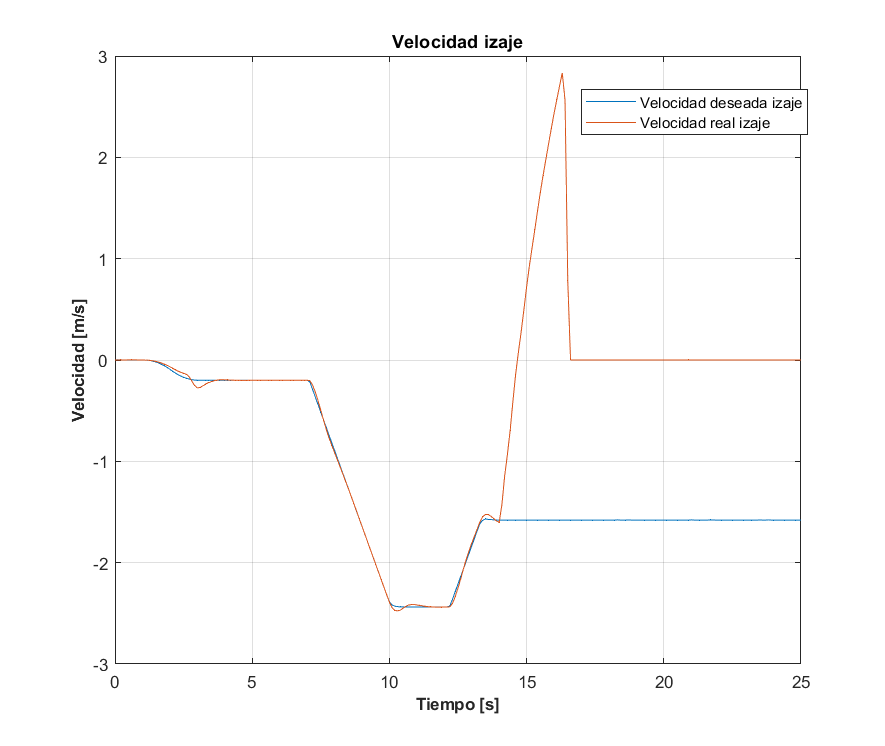
\includegraphics[width=0.75\textwidth]{images/Freno_sobrevelocidad/velocidad_izaje.png}
	\caption{Velocidad del izaje. Alerta accionada por sobrevelocidad.}
	\label{fig:sobrevelocidad_velocidad_izaje}
\end{figure}

\begin{figure}[!h]
	\centering
	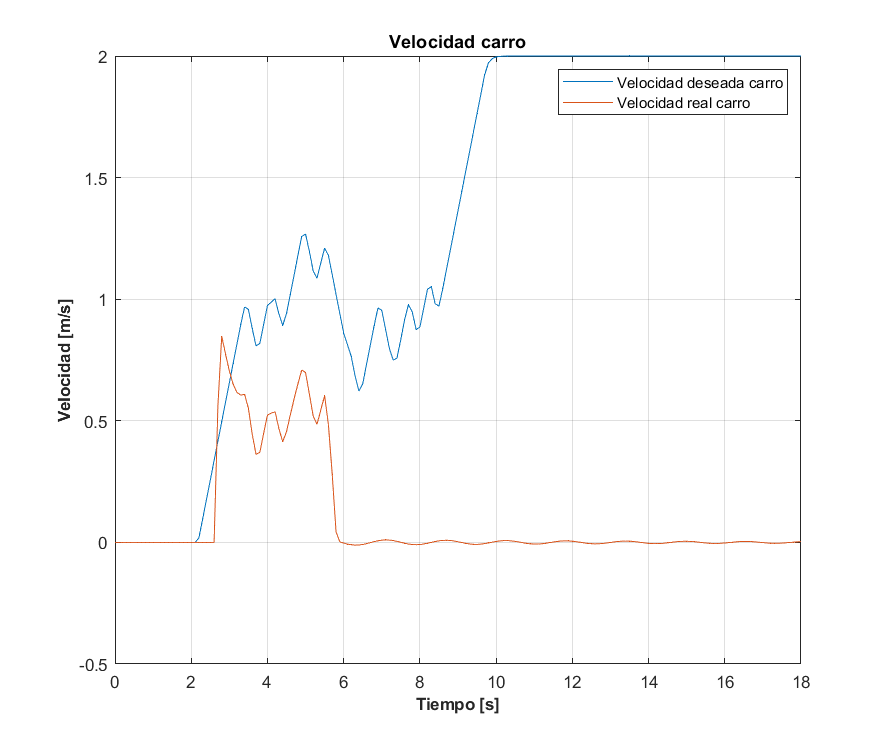
\includegraphics[width=0.75\textwidth]{images/Freno_sobrevelocidad/velocidad_carro.png}
	\caption{Velocidad del carro. Alerta accionada por sobrevelocidad.}
	\label{fig:sobrevelocidad_velocidad_carro}
\end{figure}

\begin{figure}[!h]
	\centering
	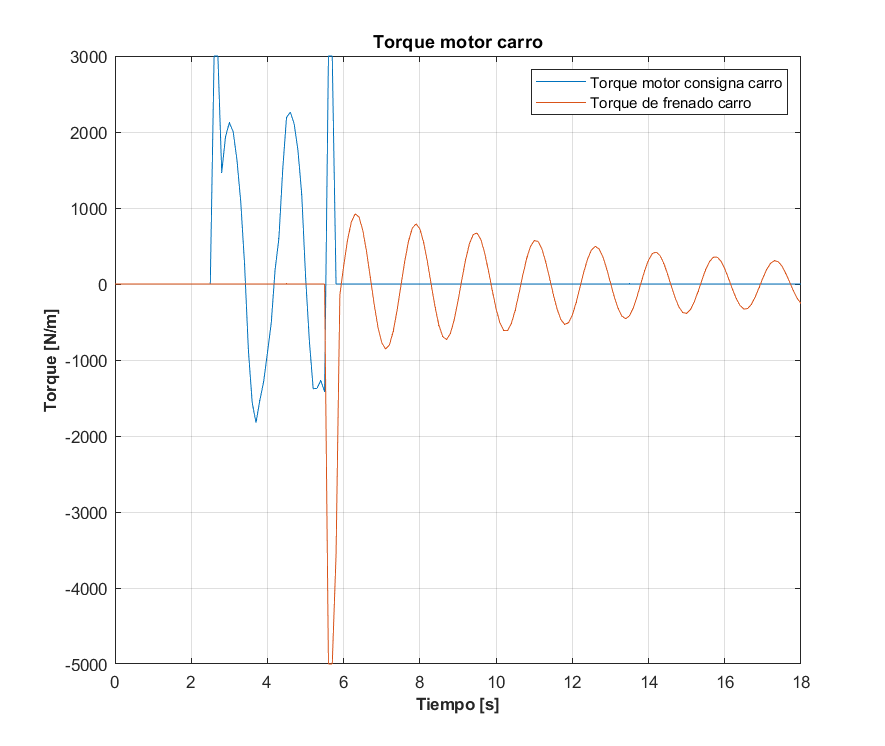
\includegraphics[width=0.75\textwidth]{images/Freno_sobrevelocidad/torque_motor.png}
	\caption{Torque de frenado del carro. Alerta accionada por sobrevelocidad.}
	\label{fig:sobrevelocidad_torque_motor_carro}
\end{figure}

\begin{figure}[!h]
	\centering
	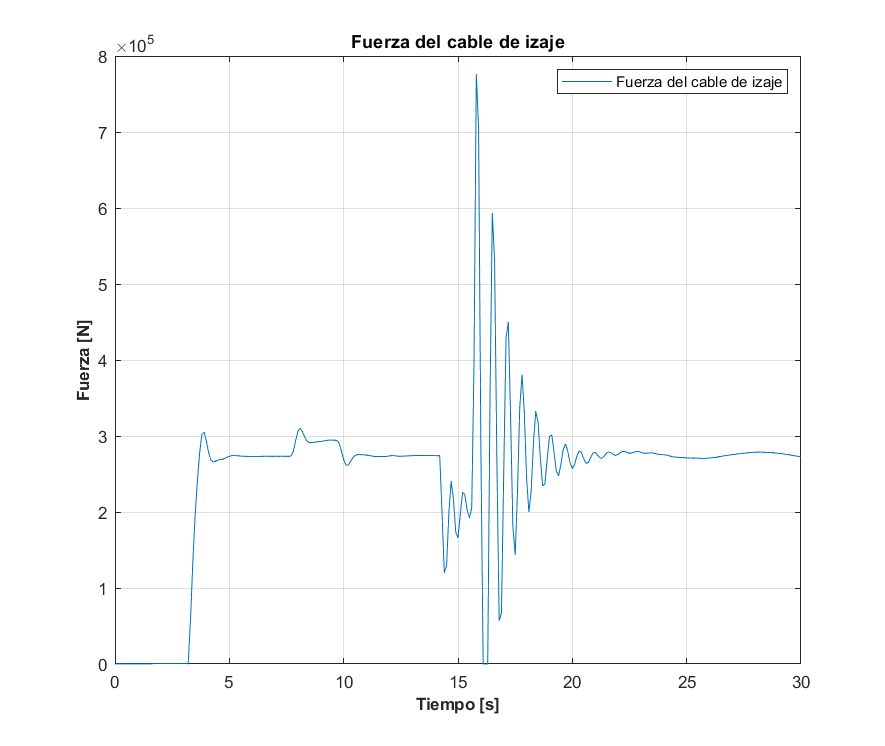
\includegraphics[width=0.75\textwidth]{images/Freno_sobrevelocidad/fuerza_cable.png}
	\caption{Fuerza del cable del izaje. Alerta accionada por sobrevelocidad.}
	\label{fig:sobrevelocidad_fuerza_cable_izaje}
\end{figure}

\newpage

Como último caso, veremos como se comporta el sistema ante una situación de \textbf{sobrepeso en la carga}. Lo que supone un riesgo tanto para el sistema como para los operarios ya que si la carga excede lo permitido se podrían sufrir daños estructurales, en los sistemas de transmisión o incluso cortarse los cables de izaje provocando una caída de la carga. Para proteger al sistema ante estas situaciones, hay un algoritmo de control que durante el pesaje de la carga, si detecta que es mayor a la permitida, se activará una alarma automáticamente. El sistema además sólo le dejará al operario bajar la carga. No se le permite subir la misma ni desplazar el carro. Esto se puede ver en las figuras \ref{fig:sobrepeso_pesaje} a \ref{fig:sobrepeso_velocidad_izaje}.

\begin{figure}[!h]
	\centering
	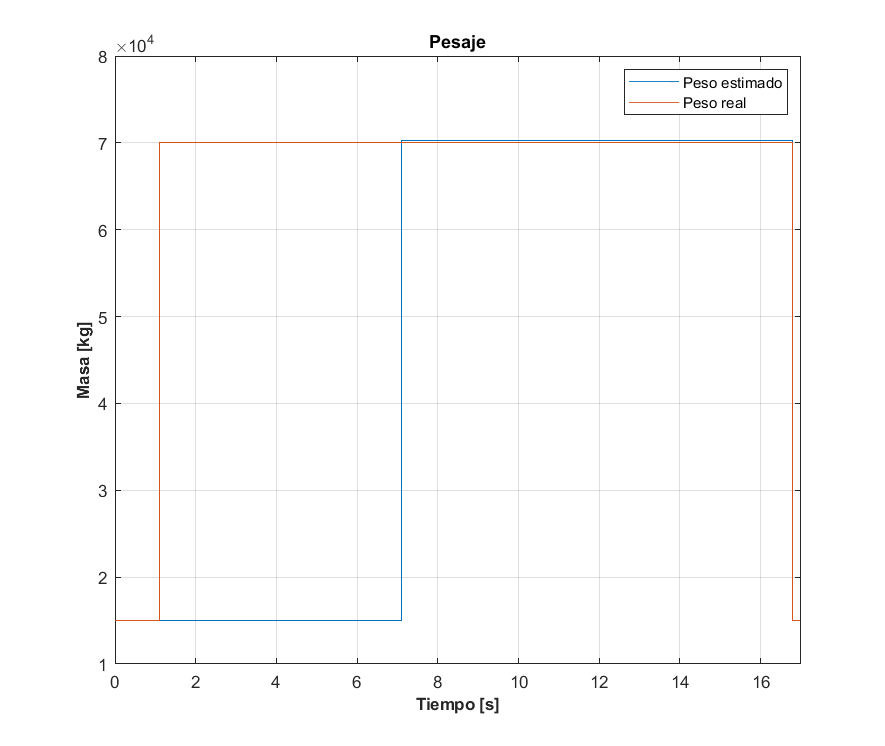
\includegraphics[width=0.75\textwidth]{images/sobrepeso/pesaje.png}
	\caption{Pesaje. Alerta accionada por sobrepeso.}
	\label{fig:sobrepeso_pesaje}
\end{figure}

\begin{figure}[!h]
	\centering
	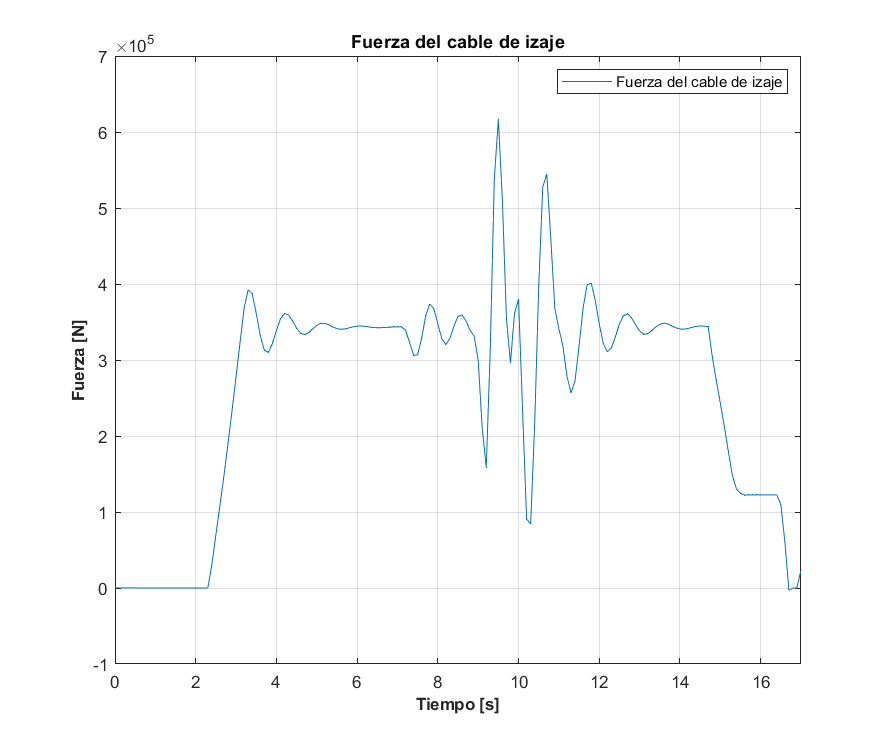
\includegraphics[width=0.75\textwidth]{images/sobrepeso/fuerza_cable.png}
	\caption{Fuerza del cable de izaje. Alerta accionada por sobrepeso.}
	\label{fig:sobrepeso_fuerza_cable}
\end{figure}

\begin{figure}[!h]
	\centering
	\includegraphics[width=0.75\textwidth]{images/sobrepeso/velocidad_izaje.png}
	\caption{Velocidad del izaje. Alerta accionada por sobrepeso.}
	\label{fig:sobrepeso_velocidad_izaje}
\end{figure}

\newpage

\section{Implementación en CODESYS}

Una vez llevada a cabo la implementación de la planta y los niveles de control 1, 2 y 3 mencionados en Simulink, se procedió a migrar los autómatas a Codesys, utilizando los lenguajes de programación gráficos SFC (``Sequential Function Chart'') y ST (``Structured Text'') de acuerdo con la norma IEC 61131-3. Es importante destacar que la implementación en Codesys se basó en el sistema implementado en Stateflow, ambos son equivalentes y siguen la misma lógica. Sin embargo, debido a que Simulink es más flexible en el diseño de autómatas, se realizaron adaptaciones para algunos estados con el objetivo de obtener un resultado similar en SFC.

\subsection{Codesys Nivel 1: Control supervisor global}

En el nivel 1 del control supervisor global, se operan ocho etapas en paralelo: \textbf{Marcha, Cable Flojo, Longitud Lh, Pos Container, Freno, Control Balanceo, Frenado Seguridad}, lo que es análogo a los 8 estados mencionados en la \ref{fig:nivel_1}. La etapa de Marcha selecciona alternativamente el modo de operación Manual (Hybrid Manual) o Automático (Automatic).

\begin{figure}[!h]
	\centering
	\includegraphics[width=0.8\textwidth]{images/codesys_nivel_1.png}
	\caption{Diagrama de Codesys del \textbf{Nivel 1}.}
	\label{fig:codesys_nivel_1}
\end{figure}

El modo Manual se utiliza para los inicios de la trayectoria y para maniobras de aproximación, mientras que el Modo Automático se encarga de las maniobras principales de traslación e izaje. Las trayectorias pueden clasificarse en ciclo simple o ciclo doble, dependiendo de si se desea cargar solamente o complementar este proceso con uno de descarga del barco. Las otras etapas son funciones auxiliares al funcionamiento de ese modo principal. Se ejecuta todo en paralelo y se encargan de ver cuándo activar el control de balanceo, cuando activar los frenos, la medición de la longitud del péndulo, detección del cable flojo, etc.

Para ver los detalles de la implementación de cada etapa, ver las figuras \ref{fig:codesys_nivel_1_marcha} a \ref{fig:codesys_nivel_1_frenado_seguridad}.

\begin{figure}[!h]
	\centering
	\includegraphics[width=0.45\textwidth]{images/codesys_nivel_1_marcha.png}
	\caption{Diagrama de Codesys de la rutina de \textbf{Marcha} del \textbf{Nivel 1}.}
	\label{fig:codesys_nivel_1_marcha}
\end{figure}

\begin{figure}
	\centering
	\includegraphics[width=0.5\textwidth]{images/codesys_nivel_1_marcha_carga.png}
	\caption{Diagrama de Codesys de la rutina de \textbf{Marcha /\ Carga} del \textbf{Nivel 1}.}
	\label{fig:codesys_nivel_1_marcha_carga}
\end{figure}

\begin{figure}
	\centering
	\includegraphics[width=0.35\textwidth]{images/codesys_nivel_1_marcha_operacion.png}
	\caption{Diagrama de Codesys de la rutina de \textbf{Marcha /\ Operación} del \textbf{Nivel 1}.}
	\label{fig:codesys_nivel_1_marcha_operacion}
\end{figure}

\begin{figure}
	\centering
	\includegraphics[width=1\textwidth]{images/codesys_nivel_1_marcha_operacion_modo.png}
	\caption{Diagrama de Codesys de la rutina de \textbf{Marcha /\ Operación /\ Modo} del \textbf{Nivel 1}.}
	\label{fig:codesys_nivel_1_marcha_operacion_modo}
\end{figure}

\begin{figure}
	\centering
	\includegraphics[width=0.2\textwidth]{images/codesys_nivel_1_marcha_operacion_trayectoria.png}
	\caption{Diagrama de Codesys de la rutina de \textbf{Marcha /\ Operación /\ Trayectoria} del \textbf{Nivel 1}.}
	\label{fig:codesys_nivel_1_marcha_operacion_trayectoria}
\end{figure}

\begin{figure}
	\centering
	\includegraphics[width=0.3\textwidth]{images/codesys_nivel_1_marcha_operacion_trayectoria_automatico.png}
	\caption{Diagrama de Codesys de la rutina de \textbf{Marcha /\ Operación /\ Trayectoria /\ Automático} del \textbf{Nivel 1}.}
	\label{fig:codesys_nivel_1_marcha_operacion_trayectoria_automatico}
\end{figure}

\begin{figure}
	\centering
	\includegraphics[width=0.85\textwidth]{images/codesys_nivel_1_marcha_operacion_trayectoria_automatico_calculo_pos.png}
	\caption{Diagrama de Codesys de la rutina de \textbf{Marcha /\ Operación /\ Trayectoria /\ Automático /\ Calculo Pos} del \textbf{Nivel 1}.}
	\label{fig:codesys_nivel_1_marcha_operacion_trayectoria_automatico_calculo_pos}
\end{figure}

\begin{figure}
	\centering
	\includegraphics[width=0.6\textwidth]{images/codesys_nivel_1_cable_flojo.png}
	\caption{Diagrama de Codesys de la rutina de \textbf{Cable Flojo} del \textbf{Nivel 1}.}
	\label{fig:codesys_nivel_1_cable_flojo}
\end{figure}

\begin{figure}
	\centering
	\includegraphics[width=0.4\textwidth]{images/codesys_nivel_1_longitud_lh.png}
	\caption{Diagrama de Codesys de la rutina de \textbf{Longitud Lh} del \textbf{Nivel 1}.}
	\label{fig:codesys_nivel_1_longitud_lh}
\end{figure}

\begin{figure}
	\centering
	\includegraphics[width=0.6\textwidth]{images/codesys_nivel_1_freno.png}
	\caption{Diagrama de Codesys de la rutina de \textbf{Freno} del \textbf{Nivel 1}.}
	\label{fig:codesys_nivel_1_freno}
\end{figure}

\begin{figure}
	\centering
	\includegraphics[width=0.4\textwidth]{images/codesys_nivel_1_balanceo.png}
	\caption{Diagrama de Codesys de la rutina de \textbf{Balanceo} del \textbf{Nivel 1}.}
	\label{fig:codesys_nivel_1_balanceo}
\end{figure}

\begin{figure}
	\centering
	\includegraphics[width=0.5\textwidth]{images/codesys_nivel_1_frenado_seguridad.png}
	\caption{Diagrama de Codesys de la rutina de \textbf{Frenado Seguridad} del \textbf{Nivel 1}.}
	\label{fig:codesys_nivel_1_frenado_seguridad}
\end{figure}

\newpage

\subsection{Codesys Nivel 0: Control de Seguridad o Protección}

En el Nivel 0 de Control de Seguridad o Protección, se operan dos etapas en paralelo: \textbf{Emergencia} y \textbf{Watchdog}, lo que es análogo a los dos estados mencionados en la figura \ref{fig:nivel_0}. La etapa Emergencia detecta problemas en función del valor de los sensores y los pulsadores, y consta de tres estados no concurrentes que manejan cada uno de los estados de emergencia. Por último, la etapa Watchdog se encarga de detectar errores en la ejecución del controlador, reinicios inesperados, etc. A continuación se detallan los diagramas de Codesys de cada una de las etapas mencionadas desde la figura \ref{fig:codesys_nivel_0} hasta la figura \ref{fig:codesys_nivel_0_watchdog}.

\begin{figure}[!h]
	\centering
	\includegraphics[width=0.4\textwidth]{images/codesys_nivel_0.png}
	\caption{Diagrama de Codesys del \textbf{Nivel 0}.}
	\label{fig:codesys_nivel_0}
\end{figure}

\begin{figure}[!h]
	\centering
	\includegraphics[width=1\textwidth]{images/codesys_nivel_0_emergency.png}
	\caption{Diagrama de Codesys de la rutina \textbf{Emergency} del \textbf{Nivel 0}.}
	\label{fig:codesys_nivel_0_emergency}
\end{figure}

\begin{figure}%[!h]
	\centering
	\includegraphics[width=0.7\textwidth]{images/codesys_nivel_0_emergency_fdc.png}
	\caption{Diagrama de Codesys de la rutina \textbf{Emergency /\ Fdc} del \textbf{Nivel 0}.}
	\label{fig:codesys_nivel_0_emergency_fdc}
\end{figure}

\begin{figure}
	\centering
	\includegraphics[width=0.7\textwidth]{images/codesys_nivel_0_emergency_speed_limit.png}
	\caption{Diagrama de Codesys de la rutina \textbf{Emergency /\ Speed Limit} del \textbf{Nivel 0}.}
	\label{fig:codesys_nivel_0_emergency_speed_limit}
\end{figure}

\begin{figure}
	\centering
	\includegraphics[width=0.9\textwidth]{images/codesys_nivel_0_watchdog.png}
	\caption{Diagrama de Codesys de la rutina \textbf{Watchdog} del \textbf{Nivel 0}.}
	\label{fig:codesys_nivel_0_watchdog}
\end{figure}

\subsection{Pruebas co-simulación. Servidor OPC UA.}

Luego de tener migrados los controladores de Nivel 1 y 0 a Codesys. Se realizó una simulación conjunta de los sistemas en Codesys, junto con el Nivel 2 de control y el modelo de la Planta en Simulink. Para lograr esto, se utilizó un protocolo de comunicación llamado OPC UA, que permite la comunicación de datos entre dispositivos de diferentes fabricantes. El sistema de comunicación utiliza un servidor OPC UA al que se conectan uno o más clientes OPC UA estableciendo un socket con TCP/IP. Este servidor es capaz de almacenar todas las variables del sistema en una memoria a la que pueden acceder todos los clientes, y escribir o tomar lecturas según sus derechos de acceso.

En este proyecto en particular, se simuló localmente un PLC en Codesys que contenía los niveles 0 y 1 de control (cliente), mientras que en Simulink se simuló la planta junto con el nivel 2 de control (cliente). Para lograr la comunicación entre estos diferentes módulos, se utilizó un servidor OPC UA proporcionado y ejecutado por Codesys. En la siguiente figura se puede ver un diagrama que muestra cómo funciona este sistema de simulación conjunta y cómo interactúan los diferentes módulos entre sí.

\begin{figure}[!h]
	\centering
	\includegraphics[width=0.8\textwidth]{images/co_simulacion_codesys.png}
	\caption{Esquema de comunicaciones de Co-simulación}
	\label{fig:comunicacion_servidor_opcua}
\end{figure}

En una parte del proceso, se utiliza el programa Codesys para ejecutar uno de los clientes OPC que contiene los niveles de control 0 y 1. Cuando se instala Codesys, se incluye automáticamente un servidor OPC UA que se puede acceder mediante el puerto 4840. Para permitir que el cliente escriba variables en el servidor, es necesario configurar los símbolos en Codesys y seleccionar las variables que se desean escribir. La figura 54 muestra el panel de configuración de símbolos que se utiliza para este propósito.

\begin{figure}[!h]
	\centering
	\includegraphics[width=0.6\textwidth]{images/variables_codesys.png}
	\caption{Variables compartidas por el servidor OPC UA}
	\label{fig:variables_codesys}
\end{figure}

En el proceso de co-simulación del sistema de control se utilizó la herramienta Matlab en conjunto con el protocolo de comunicación OPC UA para intercambiar información con el PLC virtual. Para lograr la conexión entre el servidor OPC UA y los bloques intérpretes de función de Matlab, se establecieron nodos de lectura-escritura que permiten el intercambio de variables con el PLC virtual. Se reemplazaron los modelos correspondientes de Simulink por dichos bloques intérpretes de función, permitiendo una conexión como cliente al servidor OPC UA.

Sin embargo, durante el proceso de co-simulación, se presentó un problema relacionado con el tiempo de lectura-escritura desde y hacia el servidor OPC. En un caso ideal, se podría establecer un tiempo de intercambio de variables muy bajo, lo que permitiría un intercambio de variables casi en tiempo real. Pero, se pudo determinar que si el tiempo de escritura al servidor es menor a $100\ ms$, el servidor no logra soportarlo y se pierde la conexión.

Otro inconveniente que se presentó en el desarrollo del sistema de control, fue que el control de nivel 2 requiere de un tiempo de muestreo elevado comparado con los demás, lo que impidió llevar a cabo su desarrollo en Codesys de nivel 2 discretizado. Debido a esta limitación, se decidió dejar el controlador en Simulink y no integrarlo al servidor OPC.

Finalmente, en las siguientes figuras se pueden observar los bloques intérpretes de funciones del nivel 1 y nivel 0 respectivamente en Simulink.

\begin{figure}[!h]
	\centering
	\includegraphics[width=0.53\textwidth]{images/matlab_codesys_nivel1.png}
	\caption{Bloque intérprete de función Nivel 1}
	\label{fig:bloque_interprete_funcion_nivel_1}
\end{figure}

\begin{figure}[!h]
	\centering
	\includegraphics[width=0.53\textwidth]{images/codesys_matlab_nivel0.png}
	\caption{Bloque intérprete de función Nivel 0}
	\label{fig:bloque_interprete_funcion_nivel_0}
\end{figure}

\newpage

\section{Conclusiones}

En conclusión, este proyecto de ingeniería fue exitoso en la aplicación práctica de los conocimientos adquiridos en las materias de ``Autómatas y Control Discreto'' así como de ``Automática y Máquinas Eléctricas'' para el modelado de sistemas físicos (electro-mecánicos). Se logró controlar de manera efectiva un sistema físico utilizando un autómata híbrido de control y supervisión, y un autómata de seguridad o protección.

Se desarrolló exitosamente el modelo físico y matemático de la planta a controlar, utilizando herramientas de física y análisis matemático adquiridas a lo largo de la carrera, lo cual permitió la consolidación de conceptos fundamentales.

En una segunda etapa, se diseñó un controlador en tiempo continuo compuesto por dos controladores PID y un PD para el seguimiento de las consignas de los accionamientos. Si bien el enfoque principal del proyecto fue el nivel de control 1 (control supervisor) y 0 (control de seguridad), el nivel 2 fue crucial para el cumplimiento de las trayectorias y consignas planificadas por el autómata, con un error mínimo. Para ello, se aplicó el método de sintonía serie para el cálculo de las constantes del controlador y la transformada de Laplace para obtener las funciones de transferencia del sistema a controlar.

En cuánto al nivel 1 se planteó un autómata híbrido de control y supervisión, de estados discretos activado por eventos. Para el nivel 0 se planteó un autómata de seguridad o protección, también de estados discretos activado por eventos, que se activa en caso de una falla en el sistema. En ambos niveles se implementó concurrencia de subrutinas. Finalmente, se implementaron los autómatas de control supervisor global y de seguridad siguiendo el lenguaje SFC en el entorno de programación industrial (CODESYS) siguiendo la norma IEC 61131-3. Además, se realizó una co-simulación entre el entorno de simulación industrial y simulink, utilizando los conceptos de ``Model-in-the-loop'' y ``Software-in-the-loop'', lo que permitió una mayor familiarización con entornos de trabajo profesional.

Como posibles mejoras, se sugiere optimizar la trayectoria para que esté más cerca de los contenedores, lo que permitiría ahorrar tiempo y energía. Además, en el caso de una parada de emergencia, se podría detener el sistema de manera más rápida al tener frenos mecánicos.

En conclusión, la realización de este proyecto fue muy beneficiosa tanto desde el punto de vista de la cátedra ``Autómatas y Control Discreto'' como para las materias previas, permitiendo afianzar conceptos previamente adquiridos que son fundamentales para la preparación para la vida profesional.

\section{Referencias}

[1] Guía del Proyecto Global Integrador 2022 Rev 0, Autómatas y Control Discreto, Profesor Ing. Gabriel Julián.

[2] Apuntes de cátedra, Autómatas y Control Discreto, Profesor Ing. Gabriel Julián.

[3] \href{https://help.codesys.com}{Sitio web de ayuda de Codesys - Automation Software for Engineering Control Systems.}

[4] \href{https://www.codesys.com/products/codesys-runtime/opc-ua.html}{Sitio de Codesys para conexión con el servidor OPC-UA.}

[5] \href{https://www.halvorsen.blog/documents/technology/opc/}{Tutorial de conexión entre Matlab y OPC.}

[6] \href{https:/https://de.mathworks.com/help/matlab/help-and-support.
html}{Sitio web de soporte de Matlab.}

[7] Norma IEC 61131-3.

\end{document}